\documentclass[11pt,a4paper]{article}
\usepackage[margin=2.3cm]{geometry}
\usepackage[T1]{fontenc}
\usepackage[utf8]{inputenc}
\usepackage{lmodern}
\usepackage{graphicx}
\usepackage{booktabs}
\usepackage{amsmath}
\usepackage{float}
\usepackage{caption}
\usepackage{enumitem}
\usepackage{xcolor}
\usepackage[colorlinks=true,linkcolor=blue!50!black,urlcolor=blue!50!black]{hyperref}
\graphicspath{{../reports/figures/}}
\setlist{nosep}
\captionsetup{font=small,labelfont=bf}
\newcommand{\code}[1]{\texttt{#1}}

\title{\textbf{Who earns more than 50K?}\\[2pt]
\large A supervised-learning proof of concept, from raw census data to a served prediction}
\author{Group 1: Lucas Petrelluzzi, Manuel Andrade, Amine Ennadzim, Gr\'egoire Mismaque\\[2pt]
\small Applied ML: Foundations, Engineering \& Evaluation (MSA-DATI07-05), Ilana Sebag}
\date{19 November 2026}

\begin{document}
\maketitle
\vspace{-1.2em}
\noindent\fbox{\parbox{\dimexpr\linewidth-2\fboxsep-2\fboxrule}{
\textbf{Dataset: Adult / Census Income} (\code{fetch\_openml(name="adult", version=2)}).\\
\textbf{Code:} \url{https://github.com/Petrel971/adult-income-ml} (public repository).\\
\textbf{Result:} a tuned gradient-boosting pipeline reaches a PR-AUC of 0.819 on the untouched test
set (no-skill: 0.239), is well calibrated (ECE 0.007), and is served behind a FastAPI endpoint.
The true-positive-rate gap between men and women falls from 0.106 to 0.013 after mitigation.}}

\section{Problem framing and EDA}

\paragraph{The five questions before modelling.}
\emph{Unit:} one row is one adult from the 1994 US census (48,842 rows, 14 features).
\emph{Target:} does the person earn more than 50,000 dollars a year? It is a self-revealing label
with no time horizon: features and label describe the same year.
\emph{Cheating:} every feature passes the prediction-time test (age, education, job, marital status
and declared capital income are known when a prediction is requested). Two columns are removed:
\code{fnlwgt}, a census sampling weight that describes the survey and not the person, and
\code{education}, the text version of \code{education-num}.
\emph{Split:} there is no date and one row per person, so no temporal or group leakage; the only
risk is duplicated records. We removed 52 exact duplicates of full raw rows, detected
\emph{before} dropping \code{fnlwgt}: after the drop, 6,374 rows share their values with another
row, but those are different people and must be kept.
\emph{No-skill baseline:} 23.9\% of people are positive, so ``always $\leq$50K'' has 76.1\% accuracy
and zero recall. Accuracy is therefore not our metric.

\paragraph{An honest split.} Stratified 60/20/20 (Table~\ref{tab:split}). Each set has one role,
fixed before any experiment, and the test set is read once, in Section~\ref{sec:models}.

\begin{table}[H]\centering\small
\begin{tabular}{lrrl}\toprule
Set & Rows & Positives & Role\\\midrule
Train & 29,274 & 23.9\% & fit, 5-fold cross-validation, Optuna tuning\\
Validation & 9,758 & 23.9\% & compare models, choose thresholds, fit calibrators and fairness thresholds\\
Test & 9,758 & 23.9\% & final numbers only\\\bottomrule
\end{tabular}
\caption{Split and role of each set.}\label{tab:split}
\end{table}

\paragraph{What the data says.} Figure~\ref{fig:eda} shows the imbalance and the sensitive
attribute: 30.4\% of men are positive against 10.9\% of women, and women are only 33\% of the rows.
The strongest driver is marital status: 44.6\% of married people living with their spouse earn more
than 50K, against 6.4\% of everyone else. Income rises with years of education, peaks around age 50,
and plateaus above 40 worked hours (Figure~\ref{fig:drivers}). Missing values exist only in
\code{workclass} (2,795), \code{occupation} (2,805) and \code{native-country} (856); the first two
are missing together, typically for people without a job, so the missingness is informative.
\code{capital-gain} is zero for 91.7\% of rows and reaches 99,999 for a few.

\begin{figure}[H]\centering
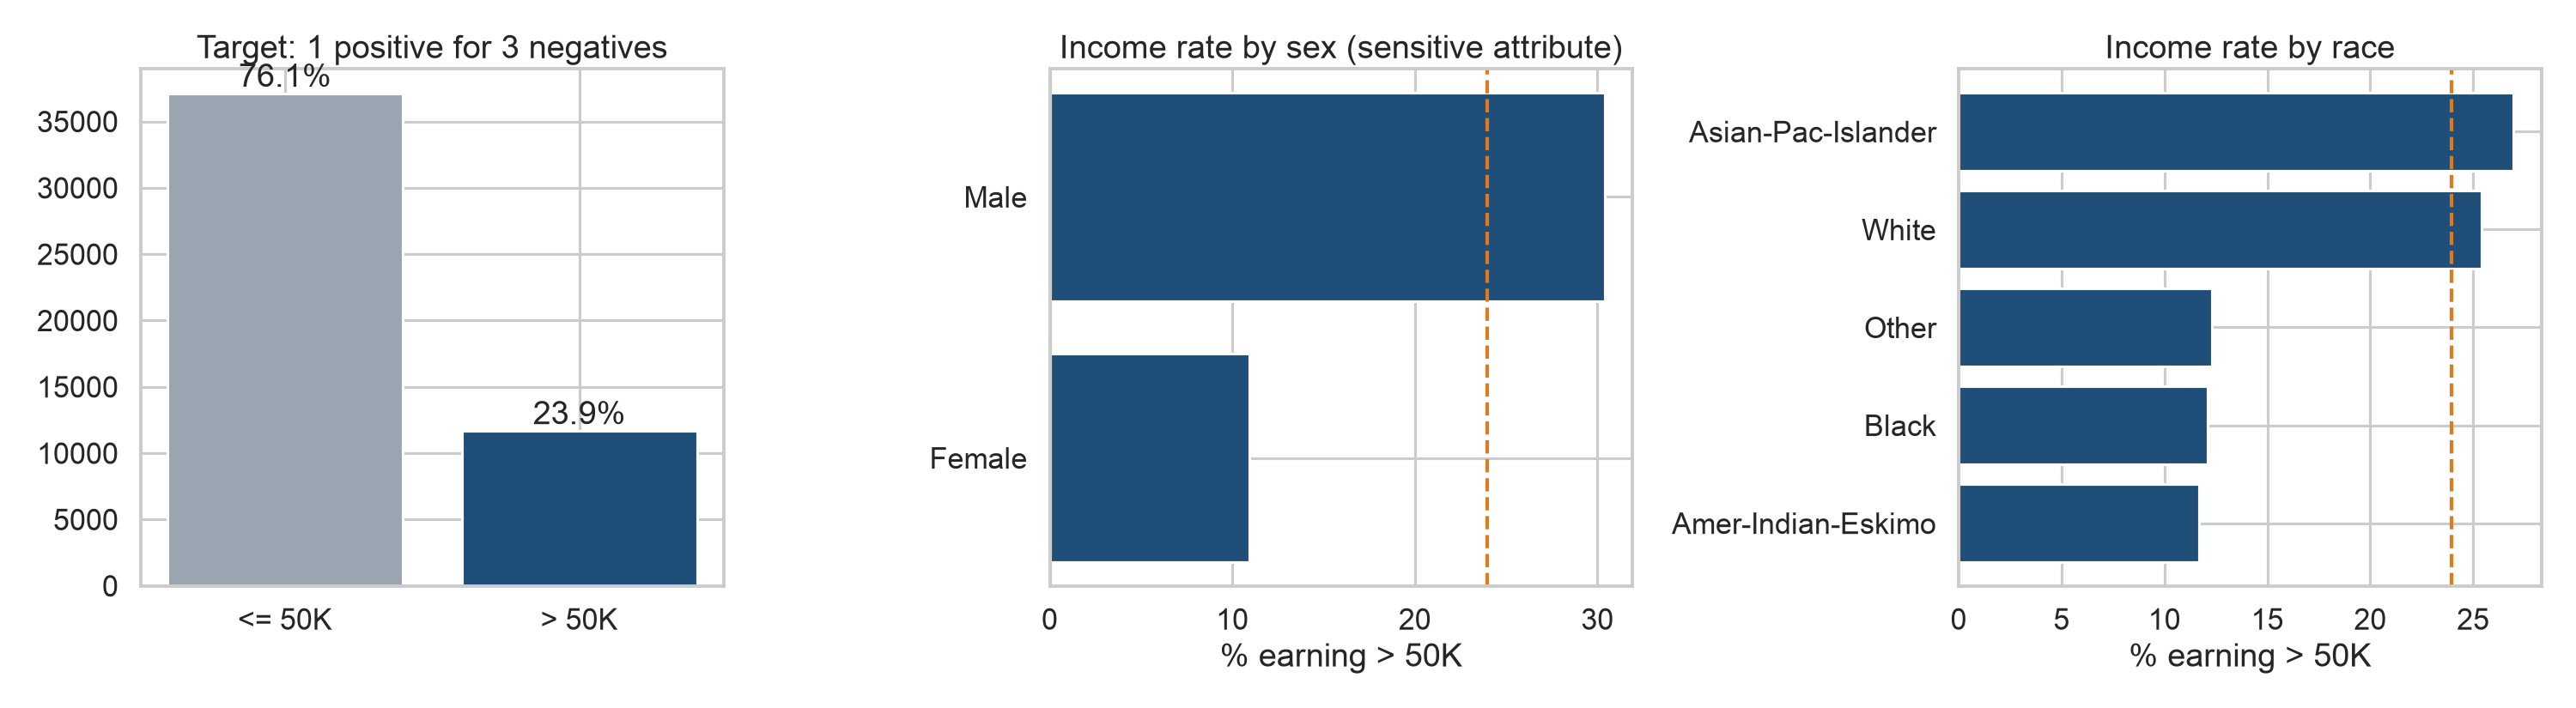
\includegraphics[width=\linewidth]{eda_target.png}
\caption{Target imbalance, and income rate by sex and by race (dashed line: overall rate).}\label{fig:eda}
\end{figure}
\begin{figure}[H]\centering
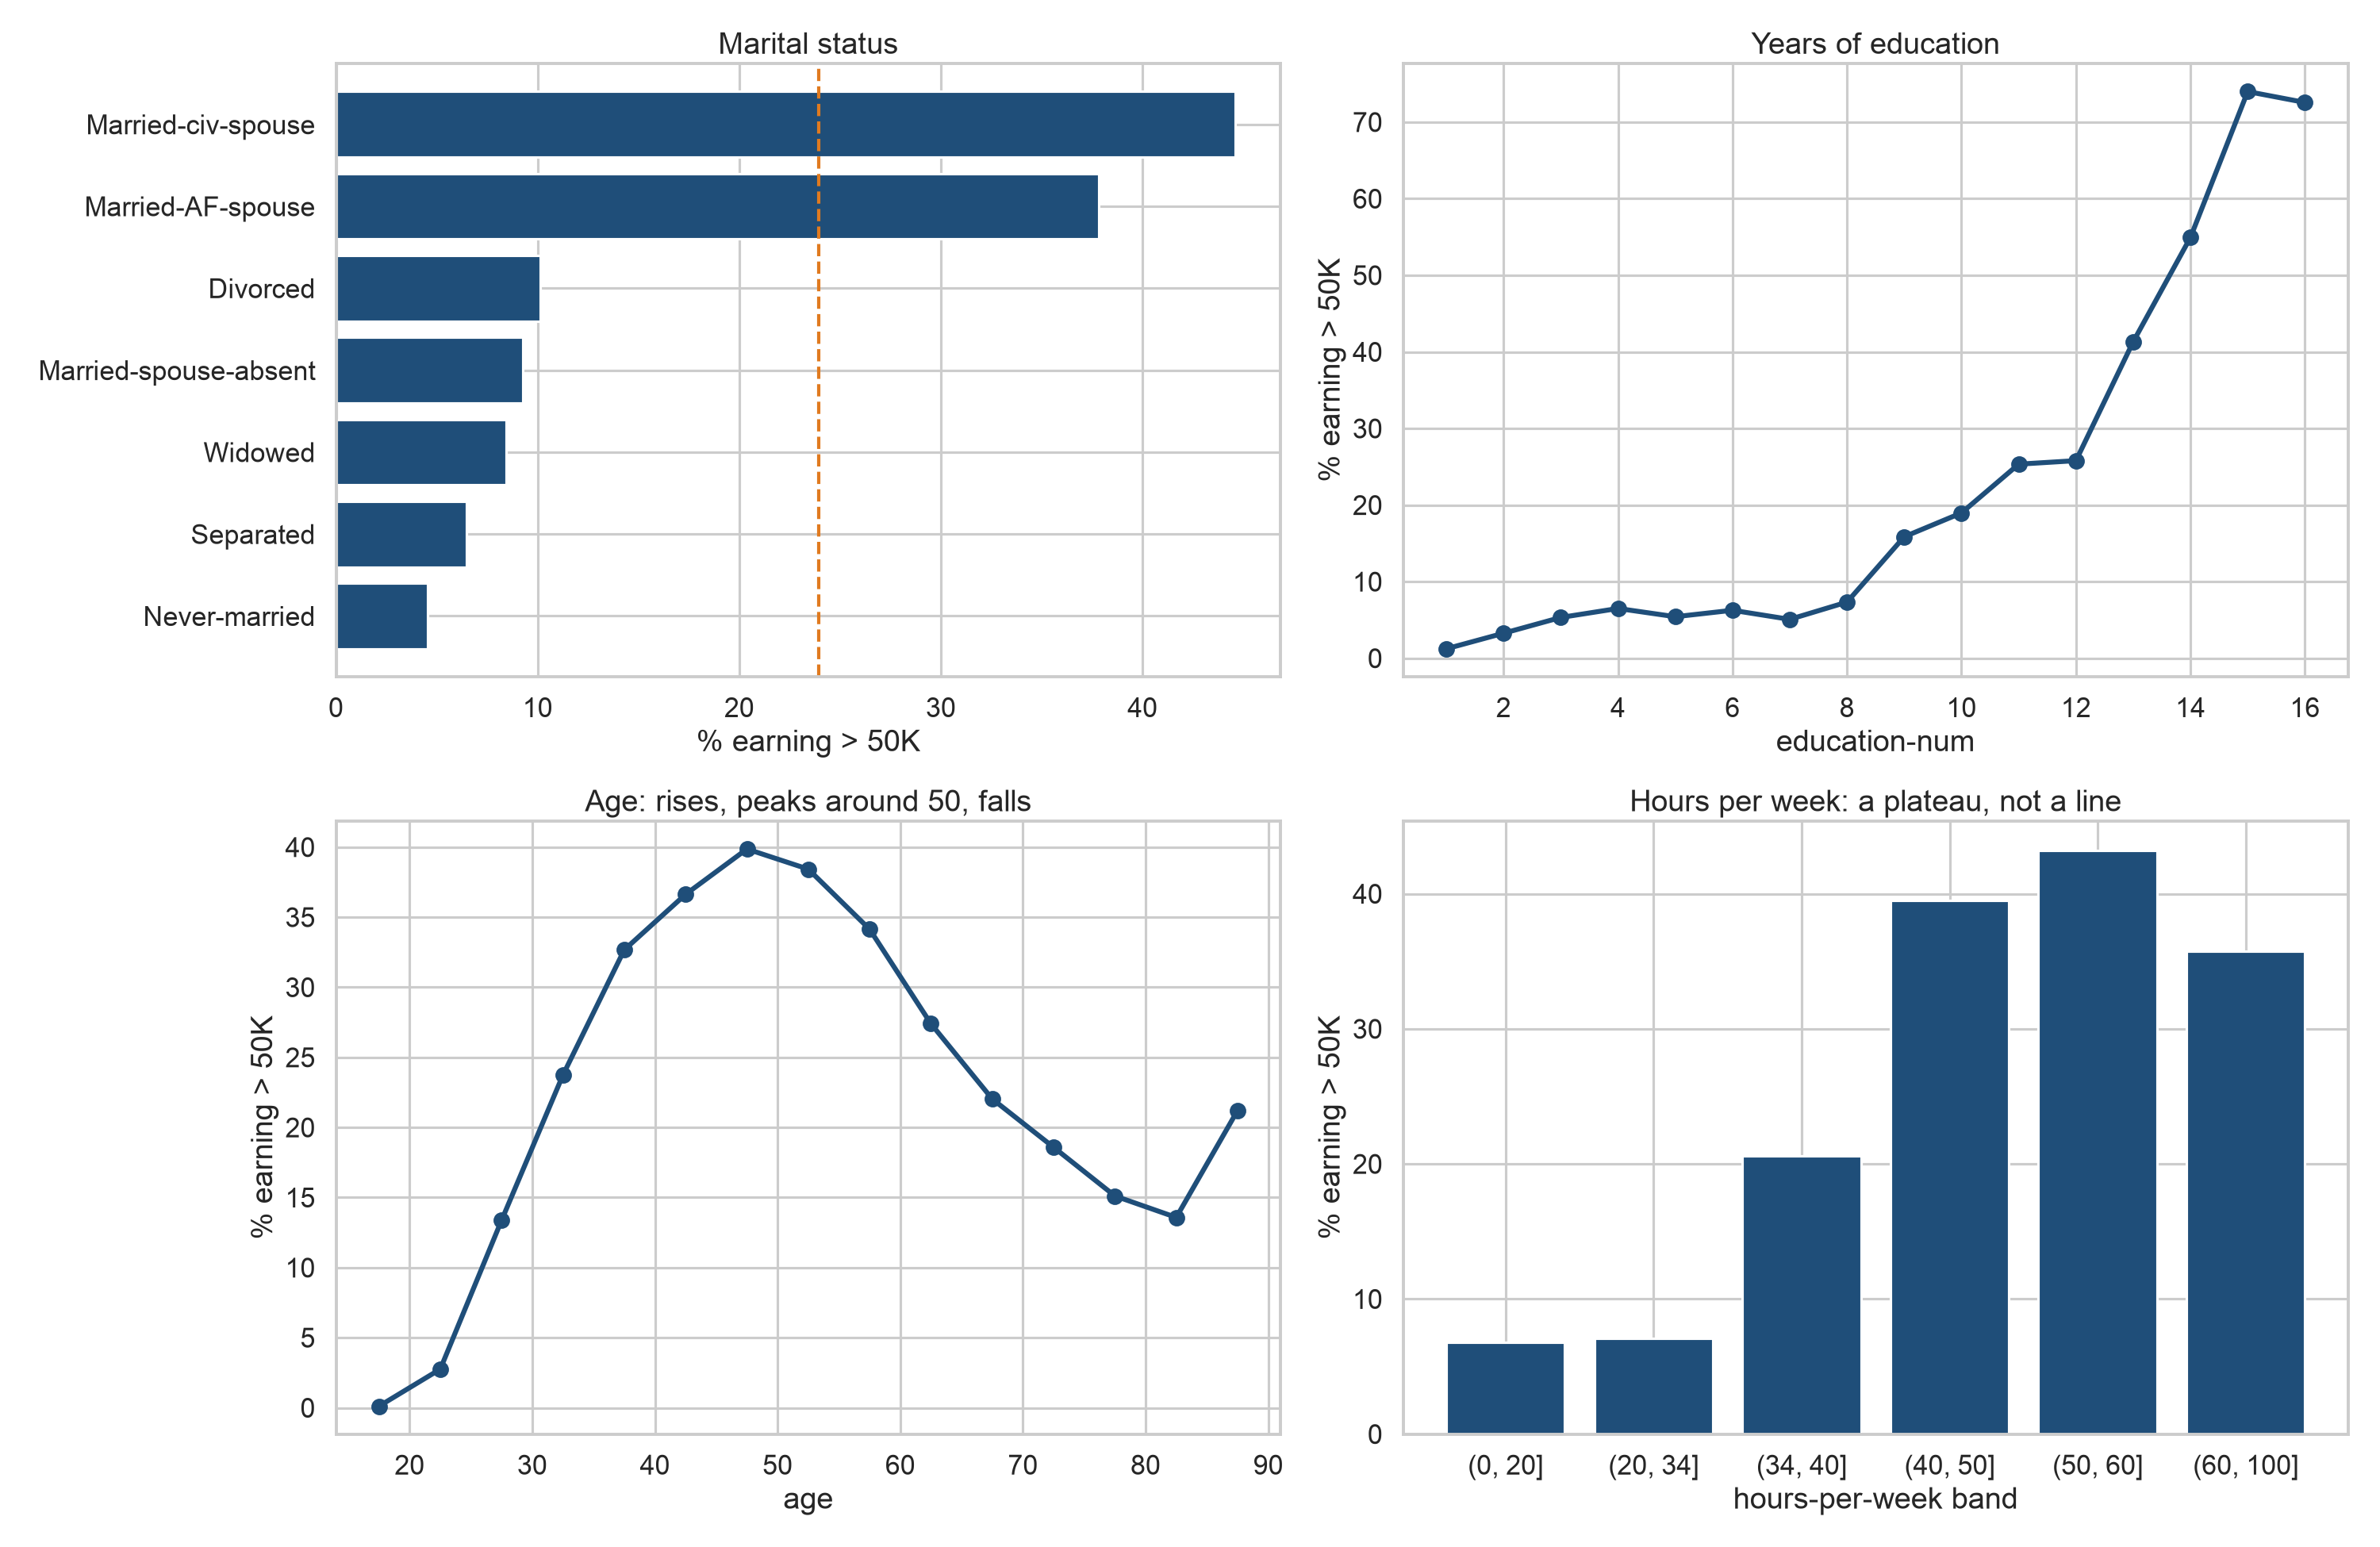
\includegraphics[width=0.86\linewidth]{eda_drivers.png}
\caption{Main drivers of income. None of the numeric effects is linear.}\label{fig:drivers}
\end{figure}

\section{Feature engineering and the single Pipeline}

\paragraph{Missing values and encoding.} Numeric columns are imputed with the median and
standardised (needed for the regularised logistic regression, harmless for trees). Categorical
columns get an explicit \code{Missing} category rather than the most frequent value, because the
missingness carries signal, then a one-hot encoding with \code{handle\_unknown="ignore"} and
\code{min\_frequency=20}, which groups rare levels. We did not use target encoding: the largest
categorical column has 41 levels, one-hot is enough and has no leakage risk.

\paragraph{Engineered features.} All are row-wise, so nothing is learned from data and nothing can leak.
\begin{itemize}
\item \code{capital\_gain\_log}, \code{capital\_loss\_log}: $\log(1+x)$ of the capital amounts. The raw
distribution has a huge tail; without the log a linear model is driven by a handful of rows.
\item \code{has\_capital}: 1 if any capital gain or loss is declared. Owning investments is a signal
in itself, whatever the amount.
\item \code{is\_married}: 1 for a married person living with their spouse. The EDA shows that the
seven marital levels reduce essentially to this contrast (44.6\% versus 6.4\%).
\item \code{hours\_band}: part-time ($<$35h), full-time (35--40h), overtime (41--59h), extreme (60h+),
to let a linear model express the plateau of Figure~\ref{fig:drivers}.
\item \code{native\_us}: 1 if born in the United States (89.8\% of rows); the 40 other countries have
too few rows each to be estimated reliably.
\end{itemize}

\paragraph{Did they help?} Table~\ref{tab:fe} is an ablation with 5-fold out-of-fold predictions on the
training set. The features buy +0.013 PR-AUC for the logistic regression, which cannot build
non-linearities itself, and almost nothing (+0.001) for gradient boosting, which finds the splits
on its own. This is the expected pattern: feature engineering matters most for the simplest model.

\begin{table}[H]\centering\small
\begin{tabular}{llrrr}\toprule
Model & Features & PR-AUC & ROC-AUC & Brier\\\midrule
Logistic regression & raw & 0.768 & 0.907 & 0.102\\
Logistic regression & engineered & \textbf{0.781} & 0.912 & 0.099\\
Gradient boosting & raw & 0.828 & 0.927 & 0.088\\
Gradient boosting & engineered & \textbf{0.830} & 0.928 & 0.088\\\bottomrule
\end{tabular}
\caption{Feature-engineering ablation (default hyperparameters, 5-fold CV on train).}\label{tab:fe}
\end{table}

\paragraph{One Pipeline.} Feature engineering, preprocessing and the model are wrapped in a single
scikit-learn \code{Pipeline} (\code{src/models.py}):
\[
\text{raw DataFrame}\;\rightarrow\;\code{FeatureEngineer}\;\rightarrow\;
\code{ColumnTransformer}\,(\text{impute, scale, one-hot})\;\rightarrow\;\text{model}\;\rightarrow\;\hat p
\]
Because the whole object is passed to cross-validation, the imputer, scaler and encoder are
re-fitted inside every training fold: validation rows never influence preprocessing. The same
object is what the endpoint loads, so serving applies exactly the training transformations.

\section{Class imbalance}\label{sec:imbalance}

\paragraph{Metrics.} With 24\% of positives we report PR-AUC (average precision) as the main ranking
metric, because its no-skill level is the prevalence (0.239) and it is not flattered by the many
negatives, together with ROC-AUC, precision, recall and F1 at the decision threshold, and the Brier
score and ECE for the quality of the probabilities. PR-AUC is also the objective of the tuning.

\paragraph{Four remedies compared.} Table~\ref{tab:imb} compares, with out-of-fold predictions on
train, (i) no remedy, (ii) class weights (\code{class\_weight="balanced"}), (iii) SMOTE, placed
inside an \code{imblearn} Pipeline so that synthetic positives are generated on the training fold
only, and (iv) threshold moving (here the threshold is picked on the same out-of-fold predictions,
so its F1 is slightly optimistic; for the final models it is picked on the validation set).

\begin{table}[H]\centering\small
\begin{tabular}{llrrrrrr}\toprule
Model & Remedy & PR-AUC & F1 & Precision & Recall & Brier & ECE\\\midrule
Logistic regression & none (threshold 0.5) & 0.781 & 0.669 & 0.740 & 0.610 & 0.099 & 0.007\\
 & class weights & 0.779 & 0.686 & 0.576 & 0.850 & 0.124 & 0.124\\
 & SMOTE & 0.780 & 0.688 & 0.581 & 0.845 & 0.123 & 0.118\\
 & threshold moving (0.36) & 0.781 & \textbf{0.700} & 0.658 & 0.748 & 0.099 & 0.007\\\midrule
Gradient boosting & none (threshold 0.5) & 0.830 & 0.715 & 0.782 & 0.658 & 0.088 & 0.005\\
 & class weights & 0.829 & 0.711 & 0.605 & 0.863 & 0.109 & 0.104\\
 & SMOTE & 0.811 & 0.710 & 0.701 & 0.719 & 0.095 & 0.028\\
 & threshold moving (0.40) & 0.830 & \textbf{0.731} & 0.723 & 0.740 & 0.088 & 0.005\\\bottomrule
\end{tabular}
\caption{Imbalance remedies, 5-fold out-of-fold predictions on the training set.}\label{tab:imb}
\end{table}

\paragraph{Reading and choice.} None of the remedies improves the ranking: PR-AUC is unchanged by
class weights and degraded by SMOTE for boosting ($-0.019$). Class weights and SMOTE only move the
operating point towards recall, which a threshold does as well, and they pay for it by distorting
the probabilities: ECE is multiplied by about 20 (0.005 to 0.104 for boosting). \textbf{We chose
threshold moving}: the model is trained on the true class proportions, keeps calibrated
probabilities, and the decision threshold is chosen on the validation set to maximise F1. It gives
the best F1 of the four options for both models. In the code, the remedy is the function
\code{best\_f1\_threshold} (\code{src/evaluate.py}), called on validation predictions in
\code{src/compare.py}; the threshold is stored with the model and applied by the endpoint.
The F1 criterion treats both errors symmetrically; with business costs for false positives and
false negatives, the same mechanism would minimise the expected cost instead.

\section{Hyperparameter tuning}

\paragraph{Protocol.} Each model is tuned with Optuna (TPE sampler, seeded) on the training set
only. A trial is one hyperparameter configuration scored by stratified 5-fold cross-validation of
the \emph{whole Pipeline}; the objective is the mean PR-AUC. Budgets: 30 trials for the logistic
regression ($C$, L1 or L2 penalty), 30 for the random forest (number of trees, depth, leaf size,
features per split) and 50 for gradient boosting (learning rate, iterations, leaves, leaf size, L2
penalty, feature subsampling): 110 trials, 550 fits.

\paragraph{Is the reported score optimistic?} The best CV score of a search is the maximum of many
noisy estimates, so it is biased upwards. We control this in two ways. First, the comparison between
models uses the validation set, which the tuning never saw. Second, for the selected model we ran a
nested cross-validation (3 outer folds, and inside each a 15-trial search with 3 inner folds): the
outer folds evaluate the whole ``tune then fit'' procedure. Nested CV gives $0.828 \pm 0.005$,
against 0.832 for the best inner score: the optimism exists but is small (0.004), and the validation
score (0.829) agrees with the nested estimate.

\paragraph{Run log.} Every trial is appended to \code{runs/run\_log.csv}: model, trial number,
parameters, mean and standard deviation of the CV PR-AUC, CV ROC-AUC and Brier, duration, and the
artifacts it corresponds to (the fitted model file of the trial and the Optuna history plot of
its study). Appendix~\ref{app:runlog} describes the file and lists the best trials.

\section{Modelling progression}\label{sec:models}

Three models of increasing flexibility, compared with the same metrics (Table~\ref{tab:val}):
a regularised \textbf{logistic regression} (linear and interpretable reference), a \textbf{random
forest} (bagging of deep trees: non-linearities and interactions, lower variance) and
\textbf{histogram gradient boosting} (shallow trees added sequentially, each correcting the errors
of the current model: lower bias). We used scikit-learn's \code{HistGradientBoostingClassifier}, the
same histogram algorithm as LightGBM, with no dependency outside scikit-learn.

\begin{table}[H]\centering\small
\begin{tabular}{llrrrrrr}\toprule
Model & Version & PR-AUC & ROC-AUC & F1 & Precision & Recall & Brier\\\midrule
No-skill & always the prior & 0.239 & 0.500 & 0.000 & 0.000 & 0.000 & 0.182\\\midrule
Logistic regression & default, $t=0.5$ & 0.776 & 0.909 & 0.663 & 0.737 & 0.603 & 0.100\\
 & tuned, $t=0.5$ & 0.778 & 0.910 & 0.663 & 0.738 & 0.602 & 0.100\\
 & tuned, $t=0.36$ & 0.778 & 0.910 & 0.698 & 0.665 & 0.734 & 0.100\\\midrule
Random forest & default, $t=0.5$ & 0.755 & 0.896 & 0.673 & 0.718 & 0.633 & 0.107\\
 & tuned, $t=0.5$ & 0.815 & 0.920 & 0.687 & 0.780 & 0.615 & 0.092\\
 & tuned, $t=0.35$ & 0.815 & 0.920 & 0.716 & 0.671 & 0.768 & 0.092\\\midrule
Gradient boosting & default, $t=0.5$ & 0.827 & 0.927 & 0.711 & 0.775 & 0.657 & 0.088\\
 & tuned, $t=0.5$ & 0.829 & 0.928 & 0.716 & 0.772 & 0.668 & 0.088\\
 & tuned, $t=0.41$ & \textbf{0.829} & \textbf{0.928} & \textbf{0.735} & 0.719 & 0.750 & \textbf{0.088}\\\bottomrule
\end{tabular}
\caption{Validation set. Thresholds $t$ are chosen on this set (maximum F1).}\label{tab:val}
\end{table}

\paragraph{What each step bought.}
\begin{itemize}
\item \emph{No-skill to logistic regression:} PR-AUC 0.239 to 0.778. Most of the signal is captured
by a linear model on well-prepared features. Tuning buys nothing (+0.002): the default $C=1$ is
already close to the optimum ($C=0.65$, L1).
\item \emph{Logistic regression to random forest:} +0.037 PR-AUC. Trees capture the age peak and
interactions such as married $\times$ education. Here tuning is essential: the default forest,
with fully grown trees, is \emph{worse} than the logistic regression (0.755) and poorly calibrated;
limiting the depth to 13 and using 43\% of the features per split brings it to 0.815.
\item \emph{Random forest to gradient boosting:} +0.014 PR-AUC and the best Brier score. Boosting
reduces the remaining bias. It is strong out of the box, so tuning buys little (+0.002), and it is
the cheapest to serve (0.6 MB on disk against 29 MB for the forest).
\item \emph{Threshold moving:} for every model, +0.019 to +0.035 F1 at no cost on ranking or calibration.
\end{itemize}

\paragraph{Final model and test results.} Gradient boosting is selected on validation PR-AUC.
Table~\ref{tab:test} gives the test results, computed once with thresholds frozen from validation.
The ordering of the three models is the same as on validation. Test scores are about 0.01 lower
than validation ones, the expected price of having selected models and thresholds on validation.
The final model finds 74\% of the high earners with 70\% precision (Figure~\ref{fig:curves}).

\begin{table}[H]\centering\small
\begin{tabular}{lrrrrrrrr}\toprule
Model & $t$ & PR-AUC & ROC-AUC & F1 & Precision & Recall & Accuracy & Brier\\\midrule
No-skill & 0.50 & 0.239 & 0.500 & 0.000 & 0.000 & 0.000 & 0.761 & 0.182\\
Logistic regression & 0.36 & 0.769 & 0.907 & 0.689 & 0.649 & 0.733 & 0.841 & 0.102\\
Random forest & 0.35 & 0.802 & 0.916 & 0.700 & 0.651 & 0.758 & 0.845 & 0.095\\
\textbf{Gradient boosting} & 0.41 & \textbf{0.819} & \textbf{0.926} & \textbf{0.720} & 0.704 & 0.736 & 0.863 & \textbf{0.090}\\\bottomrule
\end{tabular}
\caption{Untouched test set (9,758 people).}\label{tab:test}
\end{table}

\begin{figure}[H]\centering
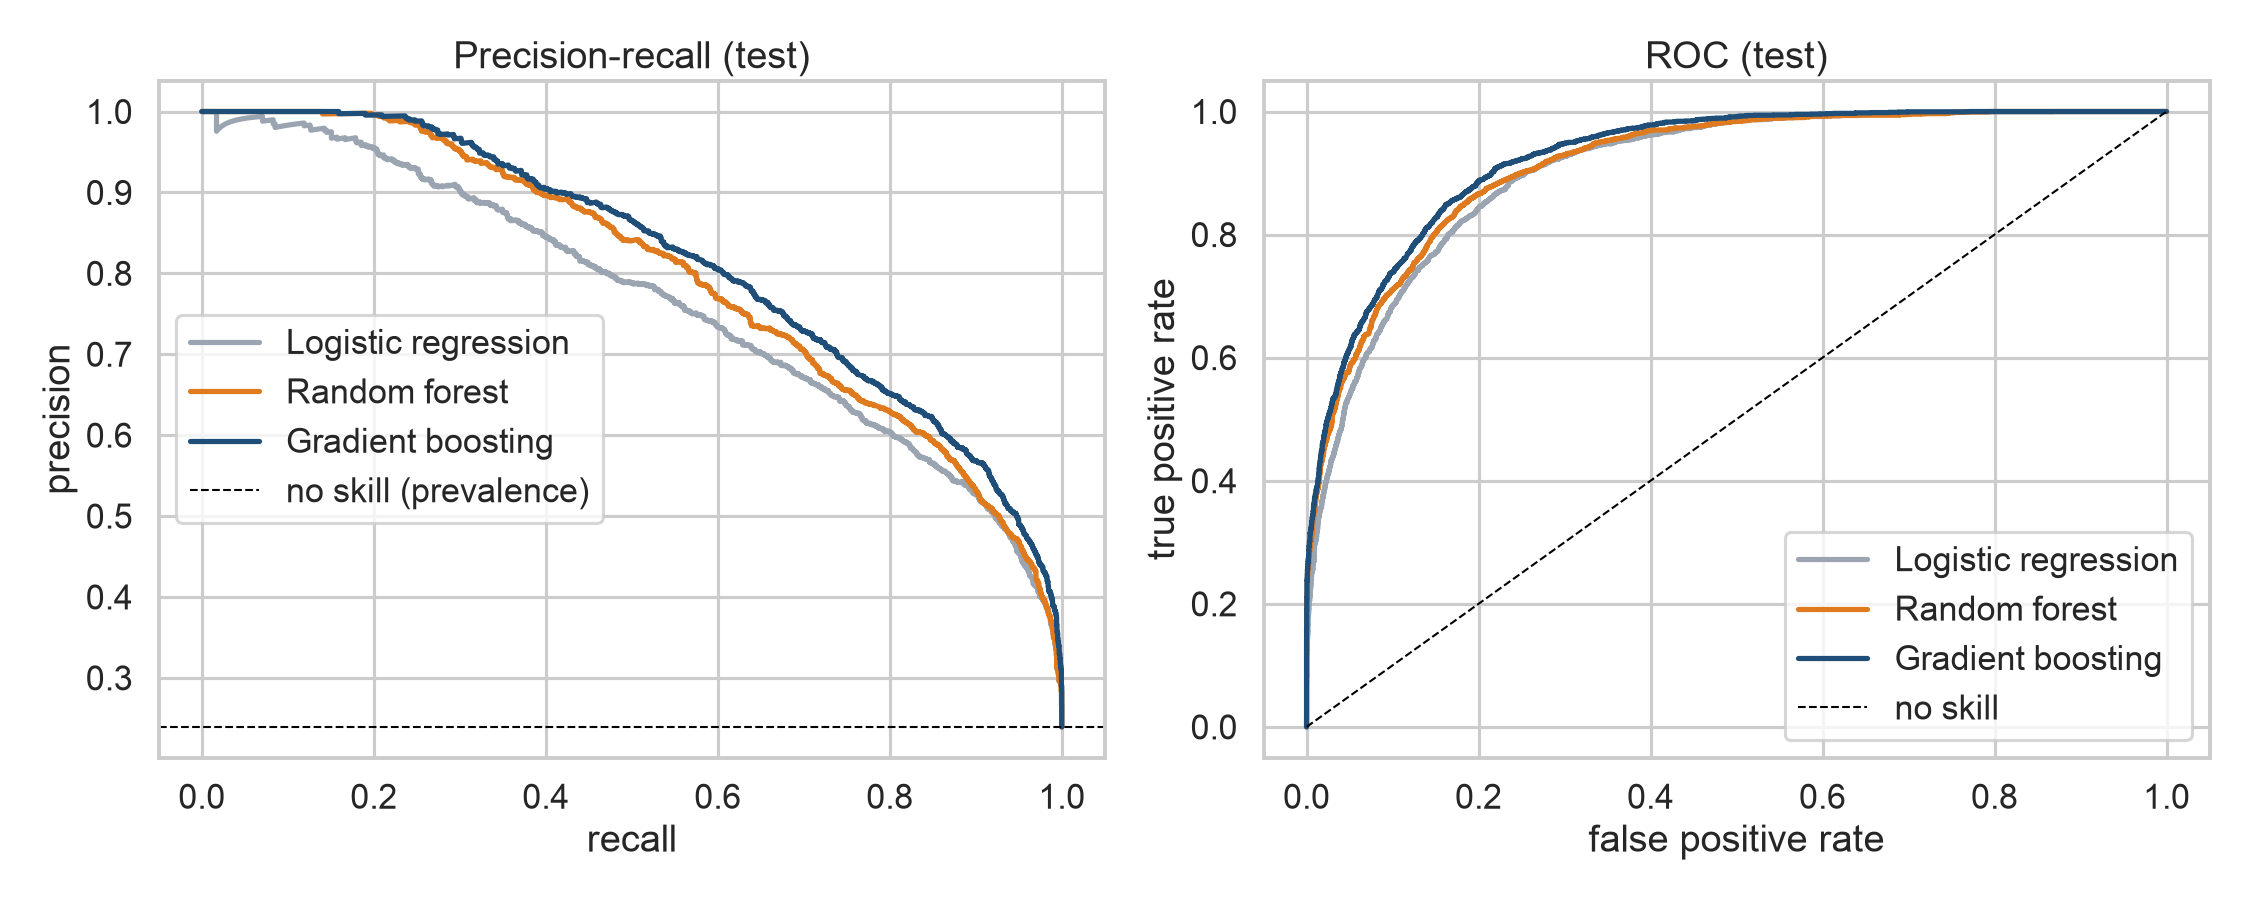
\includegraphics[width=0.62\linewidth]{pr_roc_curves.png}\hfill
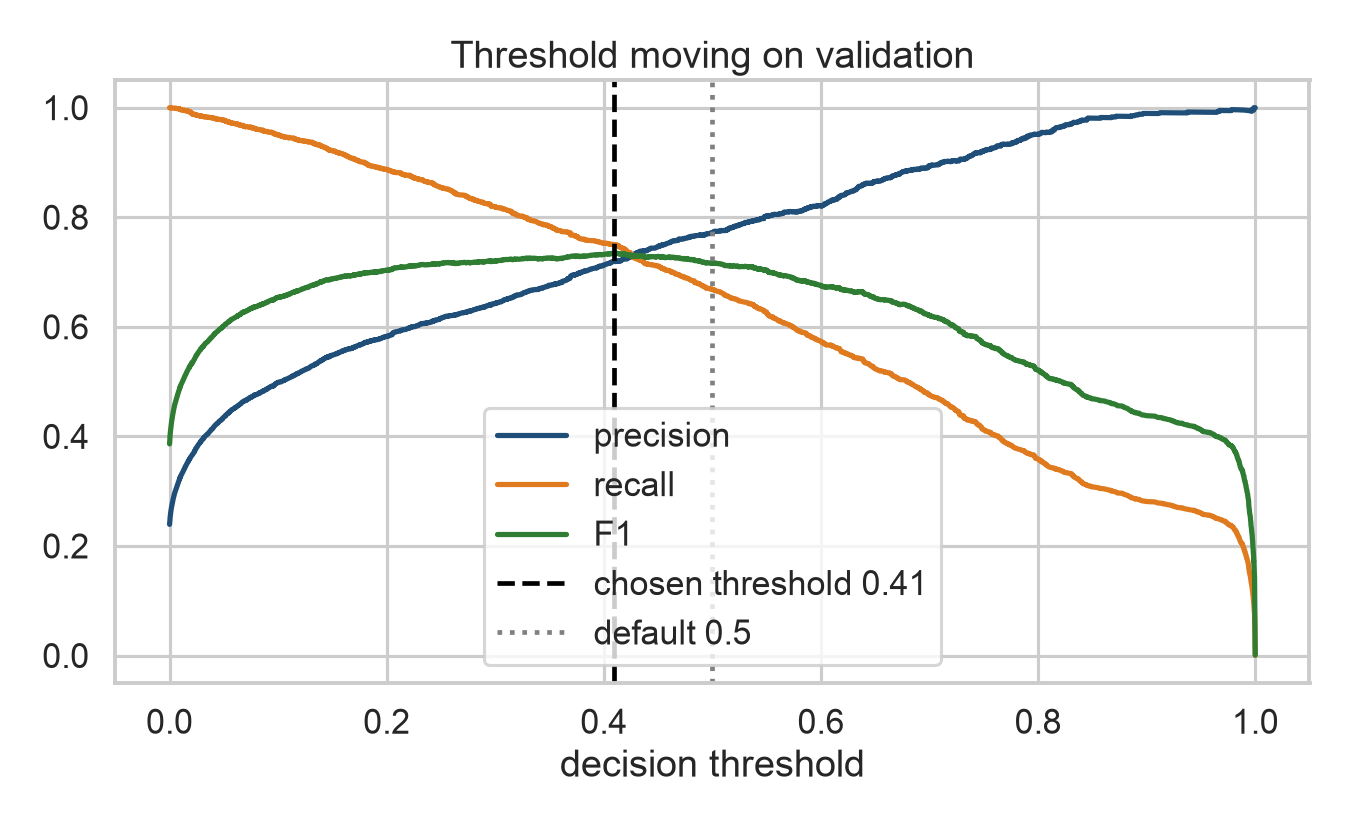
\includegraphics[width=0.36\linewidth]{threshold.png}
\caption{Left: precision-recall and ROC curves on the test set. Right: choice of the threshold of
the final model on validation.}\label{fig:curves}
\end{figure}

\section{Explainability}

\paragraph{Global.} SHAP values are computed with \code{TreeExplainer} on the validation set, in the
raw score of the model (log-odds): $f(x)=\phi_0+\sum_j \phi_j$ and $\hat p=\sigma(f(x))$, with
$\phi_0=-2.40$. Figure~\ref{fig:shap} shows the beeswarm and the mean $|\phi|$ summed over the one-hot
columns of each original feature. The five main features are age, marriage (\code{is\_married} and
\code{marital-status}), capital gain, occupation and education. As a second opinion, permutation
importance on raw validation columns (drop in PR-AUC when a column is shuffled) ranks
\code{capital-gain} (0.222), \code{marital-status} (0.103), \code{education-num} (0.056),
\code{age} (0.052) and \code{capital-loss} (0.051) first. The two methods agree on the set of
features; they differ on \code{relationship} and \code{sex}, which look unimportant under permutation
because \code{marital-status} and \code{relationship} are correlated and replace each other.

\begin{figure}[H]\centering
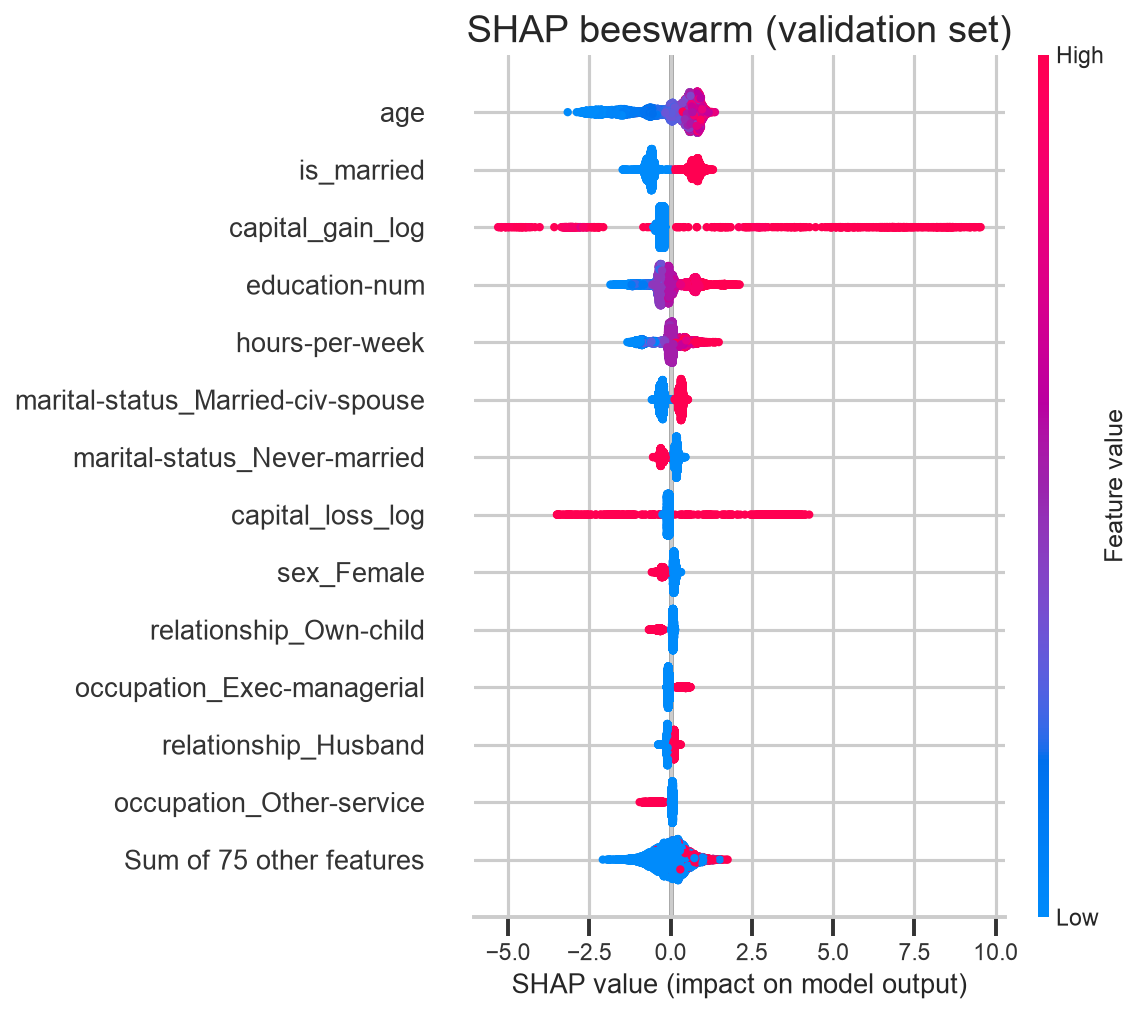
\includegraphics[width=0.53\linewidth]{shap_beeswarm.png}\hfill
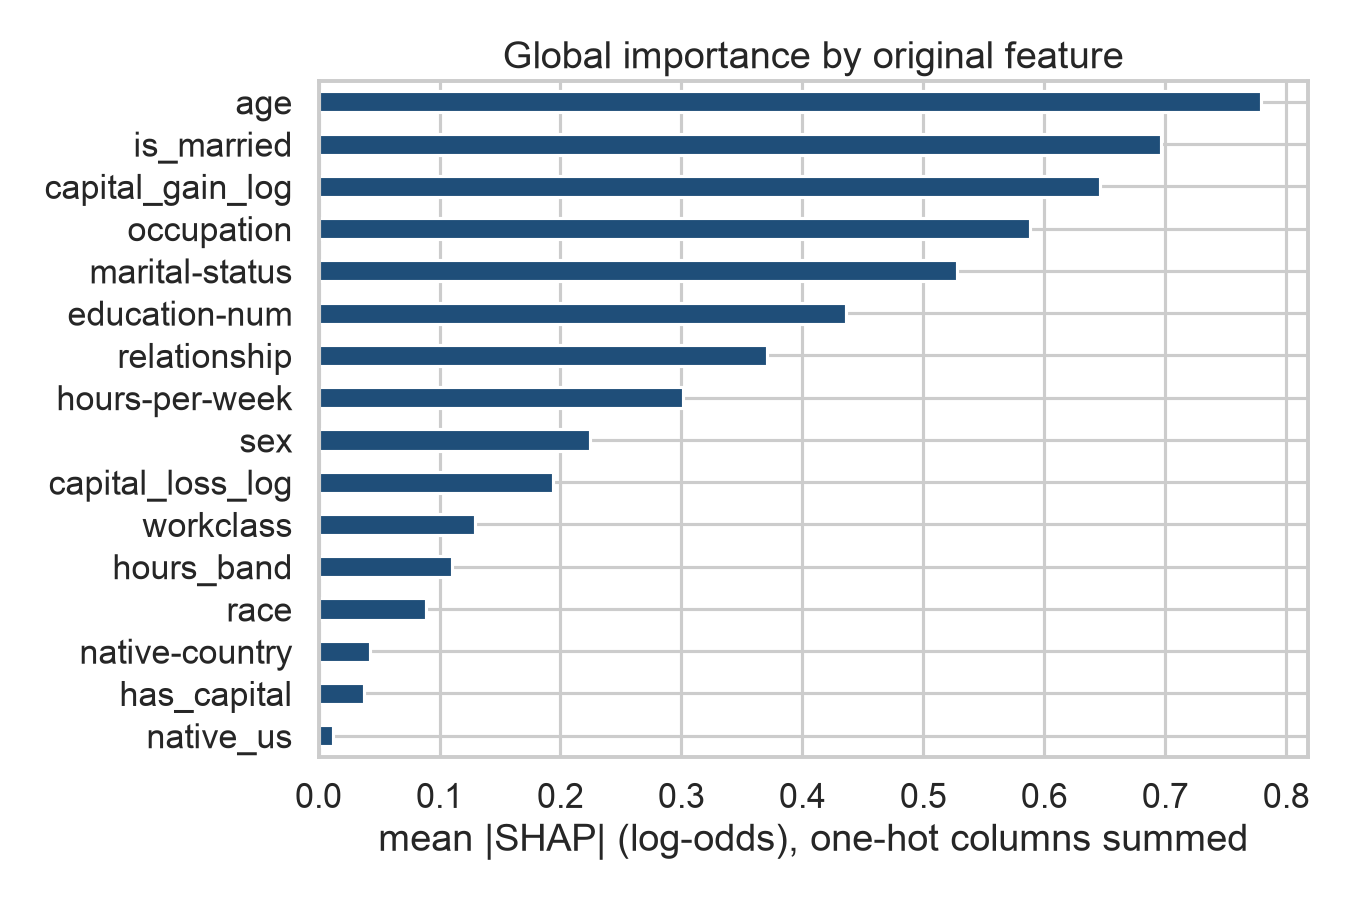
\includegraphics[width=0.45\linewidth]{shap_global.png}
\caption{Global SHAP explanations of the final model (validation set).}\label{fig:shap}
\end{figure}

\paragraph{Does it make business sense?} Mostly yes. Age stands for experience and seniority;
education and managerial or professional occupations raise the score; capital gains reveal wealth.
Three points deserve caution. (1) Marriage is not a cause of income: in 1994 census data it stands
for age, stability and household structure, and it is also a \emph{proxy for sex}
(\code{relationship = Husband / Wife}). (2) Capital gain is not monotonic: the beeswarm shows a
cluster of high values with a strongly negative contribution, i.e.\ small declared gains are
associated with low incomes; the model learned an artefact of how the census recorded gains.
(3) \code{sex\_Female} has a direct negative contribution, which motivates Section~\ref{sec:fair}.
These explanations describe the model, not the causes of income.

\paragraph{Shape of the effects.} Partial dependence and ICE curves (Figure~\ref{fig:pdp}) confirm
the EDA: the predicted probability rises with age up to about 50 and drops after 60, rises with
education with jumps around 9--10 and 13 years, and plateaus above 40--50 worked hours. For capital
gain the curve is a step: above roughly 7,000 dollars almost everyone is predicted positive, and the
dip at small values is the artefact noted above. The ICE curves are not parallel (education matters
much more for some people than for others), which reveals interactions. Caveat: a PDP forces one
value on everyone, which creates unrealistic combinations when features are correlated.

\begin{figure}[H]\centering
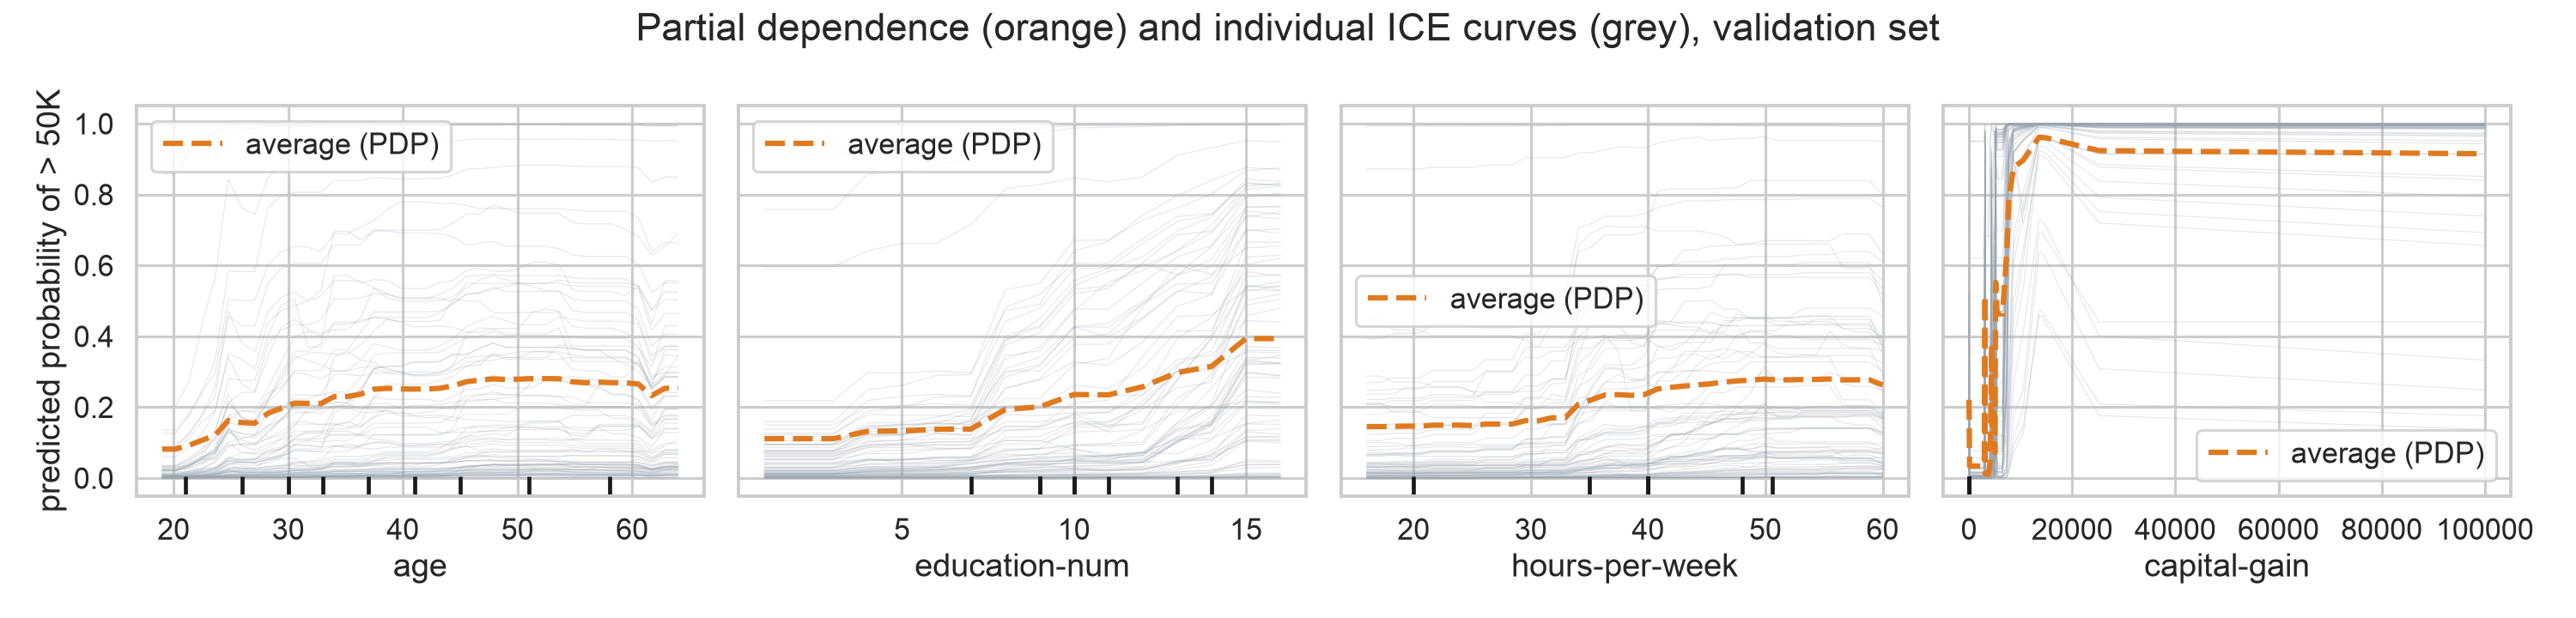
\includegraphics[width=\linewidth]{pdp.png}
\caption{Partial dependence (orange) and individual ICE curves (grey) of the final Pipeline.}\label{fig:pdp}
\end{figure}

\paragraph{Local.} Five validation predictions were explained with waterfall plots
(Figure~\ref{fig:local} and repository): a confident true positive, a confident true negative, the
most confident false positive and false negative, and a borderline case.
\begin{itemize}
\item \emph{True positive} ($\hat p=1.00$): a 30-year-old married executive with a master's degree,
60 hours a week and a capital gain of 15,024: the gain alone contributes $+8.7$ log-odds.
\item \emph{True negative} ($\hat p=0.00$): 18 years old, 4 hours a week, never married; age
($-1.8$) and a small capital gain of 594 ($-2.6$) drive the score down.
\item \emph{False positive} ($\hat p=1.00$): a self-employed married man working 90 hours with a
capital gain of 41,310 ($+7.3$) who nevertheless earns less than 50K. The model trusts capital
gains almost blindly; a one-off gain is not a salary.
\item \emph{False negative} ($\hat p=0.00$): 22 years old, 15 hours a week, no occupation recorded,
yet above 50K. Nothing in the features can explain the label: irreducible error or label noise.
\item \emph{Borderline} ($\hat p=0.41$): a 36-year-old married clerk, 40 hours, no capital:
marriage and age push up, the absence of capital gain pushes down.
\end{itemize}

\begin{figure}[H]\centering
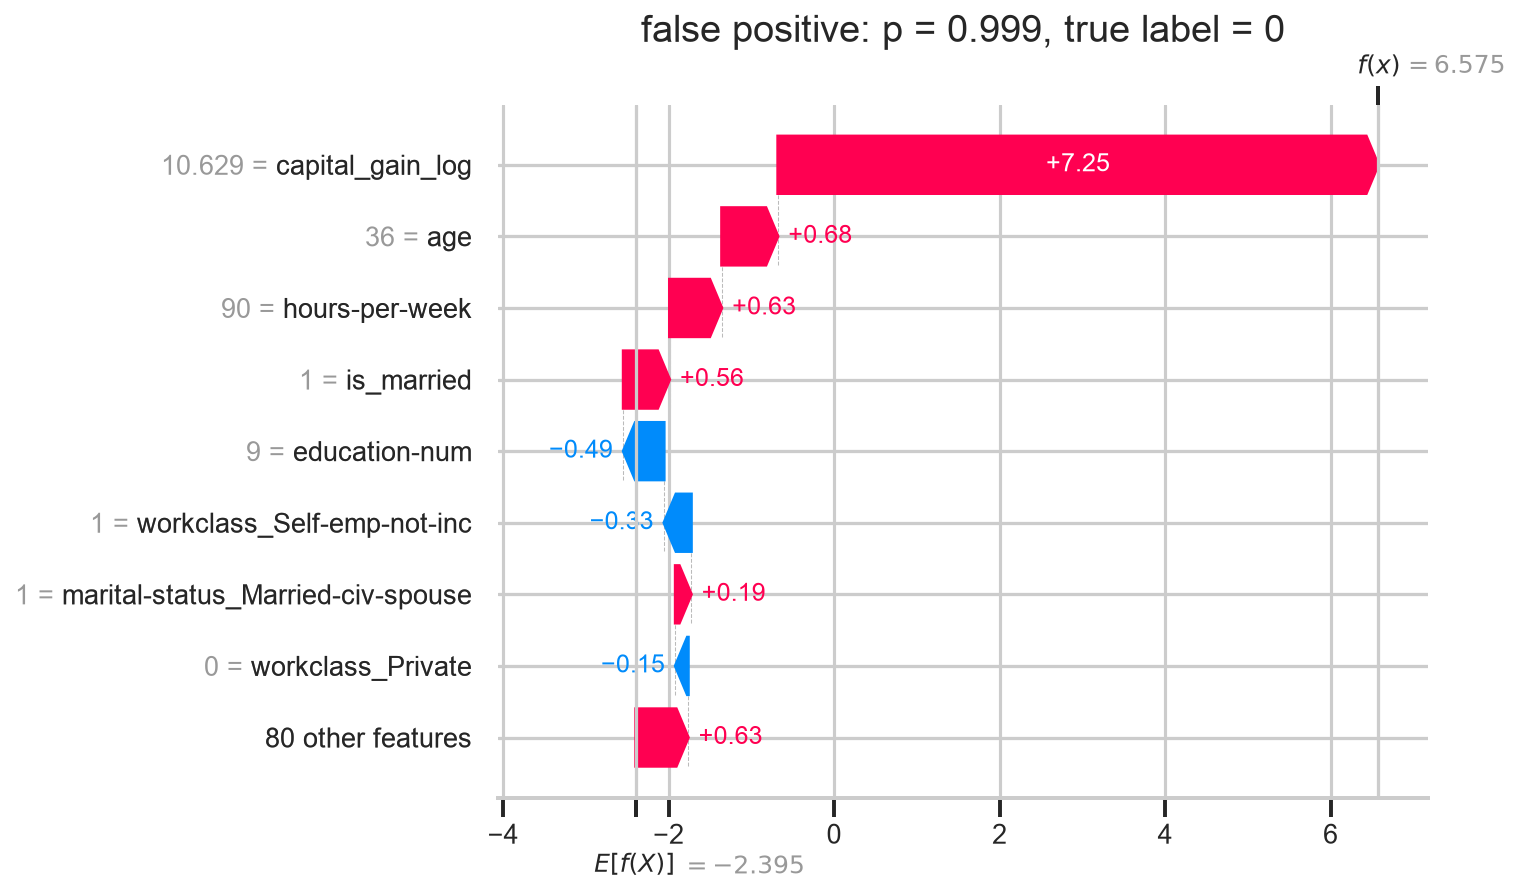
\includegraphics[width=0.49\linewidth]{shap_local_false_positive.png}\hfill
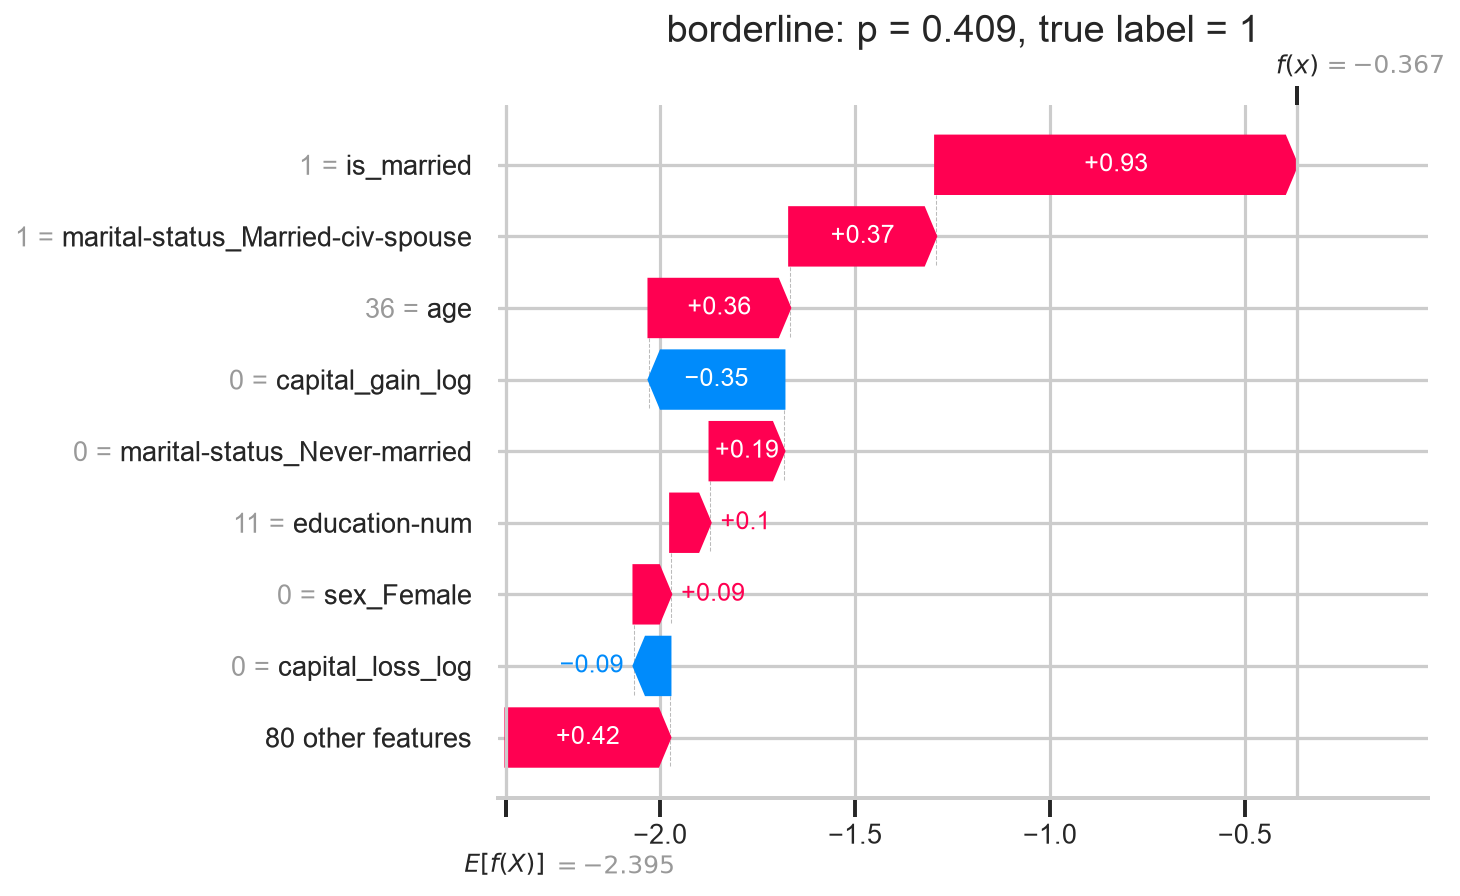
\includegraphics[width=0.49\linewidth]{shap_local_borderline.png}
\caption{Local explanations: the most confident false positive (left) and a borderline case (right).}\label{fig:local}
\end{figure}

\section{Calibration}

Figure~\ref{fig:calib} shows the reliability curve of the final model on the test set (10 bins) and
Table~\ref{tab:calib} the scores. The curve follows the diagonal: among people who receive a
probability near 0.25, 25\% are positive; near 0.75, 75\%. The largest deviations are in the bins
0.4--0.5 (0.45 predicted, 0.41 observed) and 0.8--0.9 (0.84 predicted, 0.82 observed).

\begin{table}[H]\centering\small
\begin{tabular}{lrrrr}\toprule
Model & Brier & ECE & Mean predicted & ROC-AUC\\\midrule
Final model, as is & 0.0903 & 0.0069 & 0.242 & 0.926\\
Final model + Platt scaling (fitted on validation) & 0.0902 & 0.0052 & 0.242 & 0.926\\
Final model + isotonic (fitted on validation) & 0.0905 & 0.0069 & 0.241 & 0.926\\
Same model trained with class weights & 0.1137 & 0.1101 & 0.350 & 0.926\\\bottomrule
\end{tabular}
\caption{Calibration on the test set (observed positive rate: 0.239).}\label{tab:calib}
\end{table}

\begin{figure}[H]\centering
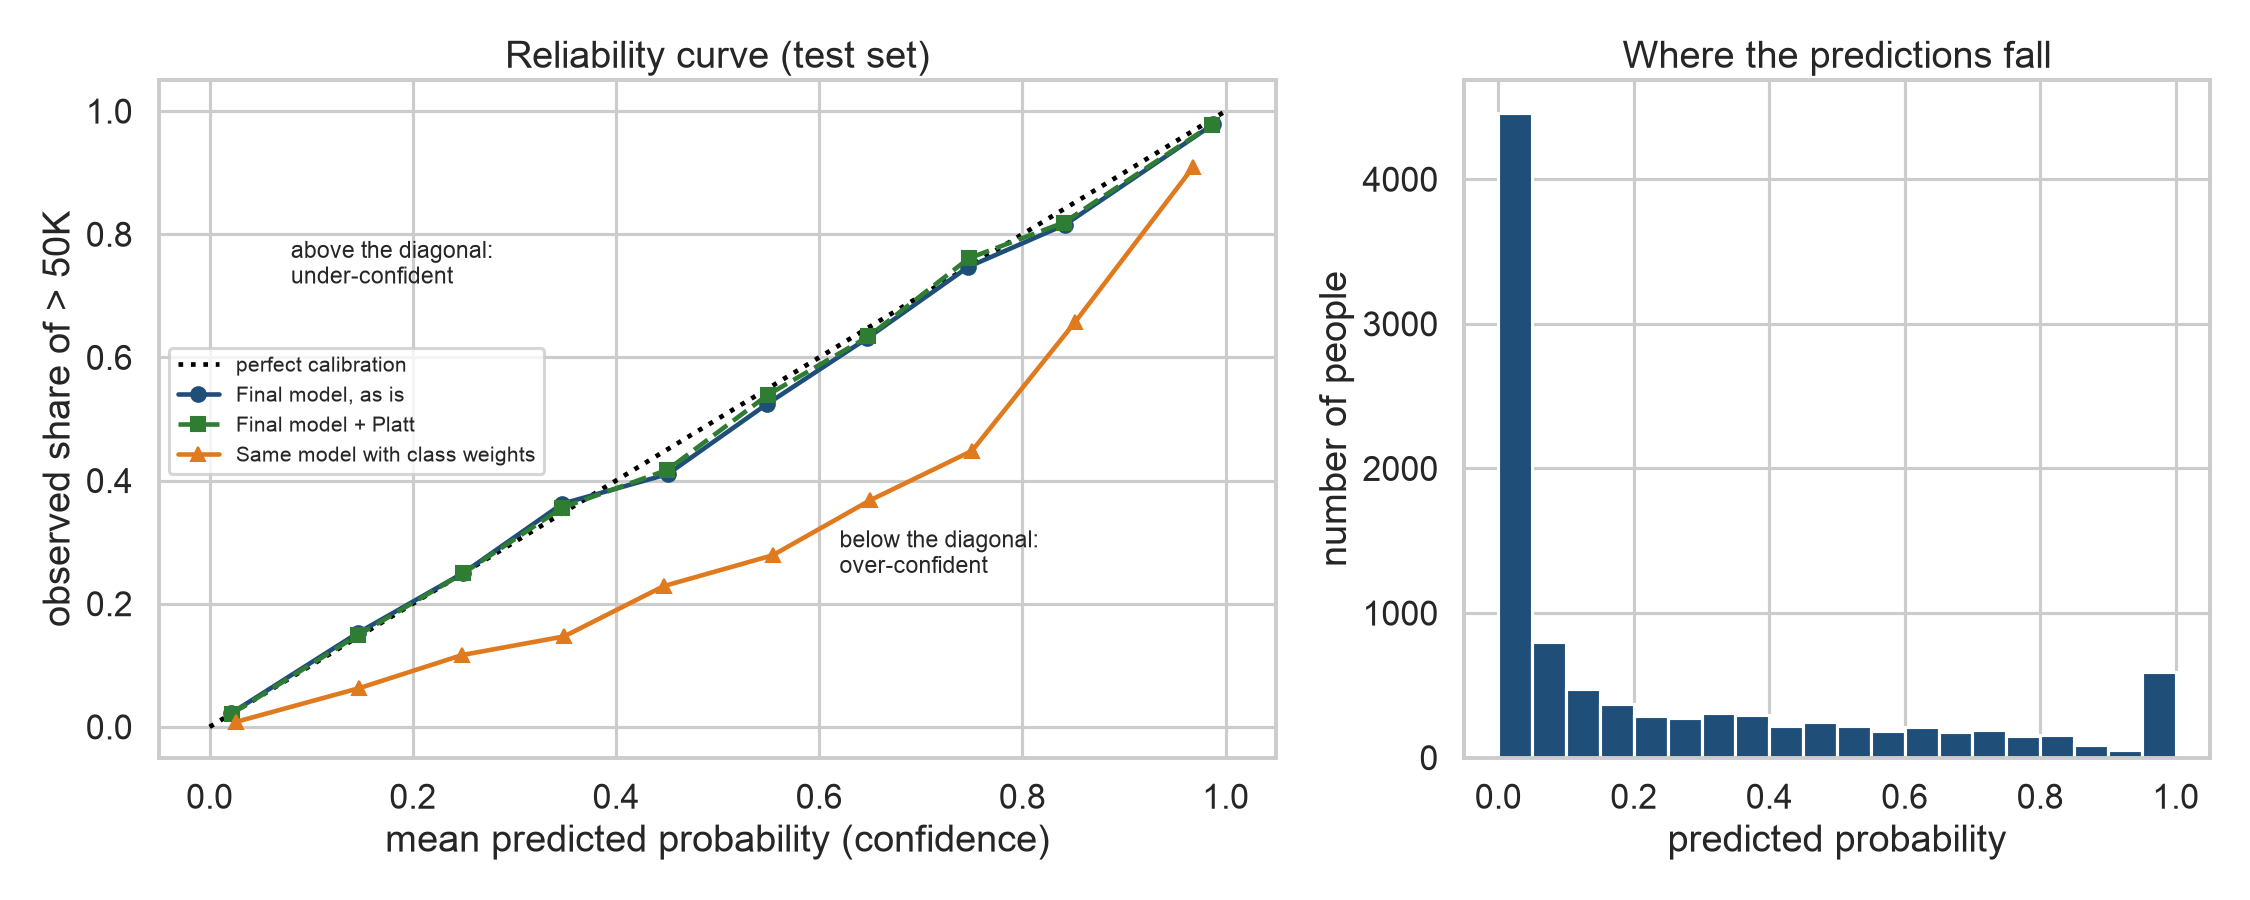
\includegraphics[width=0.9\linewidth]{calibration.png}
\caption{Reliability curve and distribution of predicted probabilities (test set).}\label{fig:calib}
\end{figure}

\paragraph{Over- or under-confident?} Very slightly \textbf{over-confident}: the mean predicted
probability is 0.242 for an observed rate of 0.239 (signed gap $+0.003$), and the deviations sit
below the diagonal in the middle bins. With an ECE of 0.007 the effect is negligible.
\paragraph{Would we trust the probabilities as is?} \textbf{Yes.} Post-hoc calibration brings no
real gain (Platt: ECE 0.0052, same Brier; isotonic leaves the ECE unchanged and slightly worsens the Brier), so the endpoint serves the raw
probabilities. Two reasons explain this: boosting minimises the log-loss, a proper scoring rule, and
we did not re-weight the classes. The last line of Table~\ref{tab:calib} is the counterfactual: the
same model with class weights has the same ROC-AUC but predicts 0.350 on average for a true rate of
0.239 (ECE 0.110, strongly over-confident). This confirms the choice of Section~\ref{sec:imbalance}.
One limit: calibration is verified on the same population; on a different year or country the
probabilities would have to be re-checked.

\section{Fairness and bias audit}\label{sec:fair}

\paragraph{Definitions.} The sensitive attribute is \code{sex} ($A$); $D$ is the decision at the
threshold and $Y$ the true label. \emph{Demographic parity}: $P(D{=}1\mid A)$ equal across groups
(gap of selection rates; the ratio is the disparate impact). \emph{Equal opportunity}:
$P(D{=}1\mid Y{=}1,A)$ equal, i.e.\ equal true positive rates. \emph{Equalized odds}: equal true
positive rates and equal false positive rates. We target \textbf{equal opportunity}: the base rates
differ strongly in the data (30.6\% of men and 10.4\% of women in the test set are positive), so
demographic parity would force many wrong decisions, whereas equal opportunity asks that a woman who
does earn more than 50K has the same chance of being recognised as a man who does.

\paragraph{Audit.} With the single threshold 0.41 (Table~\ref{tab:fair}), the model finds 75.2\% of
high-earning men but only 64.6\% of high-earning women: an equal-opportunity gap of 0.106. The
selection rates are 32.6\% and 9.8\% (ratio 0.30, far below the usual four-fifths rule), mostly
inherited from the base rates. The model is equally well calibrated in both groups (ECE 0.011 in
both): the unfairness comes from applying one threshold to two different score distributions, not
from wrong probabilities. A slice by race shows the same pattern for Black people (TPR 0.63, 923
rows); the other groups are too small to conclude (75 to 291 rows).

\paragraph{Mitigation.} We apply a post-processing technique: \textbf{one threshold per group},
chosen on the validation set. A grid search keeps the pairs of thresholds whose TPR gap is below
0.01 and takes the pair with the best F1: 0.41 for men, 0.22 for women. As a control we also tried
``fairness through unawareness'' (retraining without \code{sex}).

\begin{table}[H]\centering\small
\begin{tabular}{lrrrrrrr}\toprule
Setting & F1 & Prec. & Recall & Acc. & DP gap & EO gap & FPR gap\\\midrule
Before: single threshold & 0.720 & 0.704 & 0.736 & 0.863 & 0.228 & 0.106 & 0.103\\
Control: \code{sex} removed from the features & 0.715 & 0.706 & 0.725 & 0.862 & 0.215 & 0.085 & 0.093\\
\textbf{After: group thresholds} & 0.713 & 0.677 & 0.753 & 0.855 & 0.178 & \textbf{0.013} & 0.062\\\bottomrule
\end{tabular}
\caption{Performance and fairness gaps (male minus female) on the untouched test set.
DP: demographic parity, EO: equal opportunity.}\label{tab:fair}
\end{table}

\begin{figure}[H]\centering
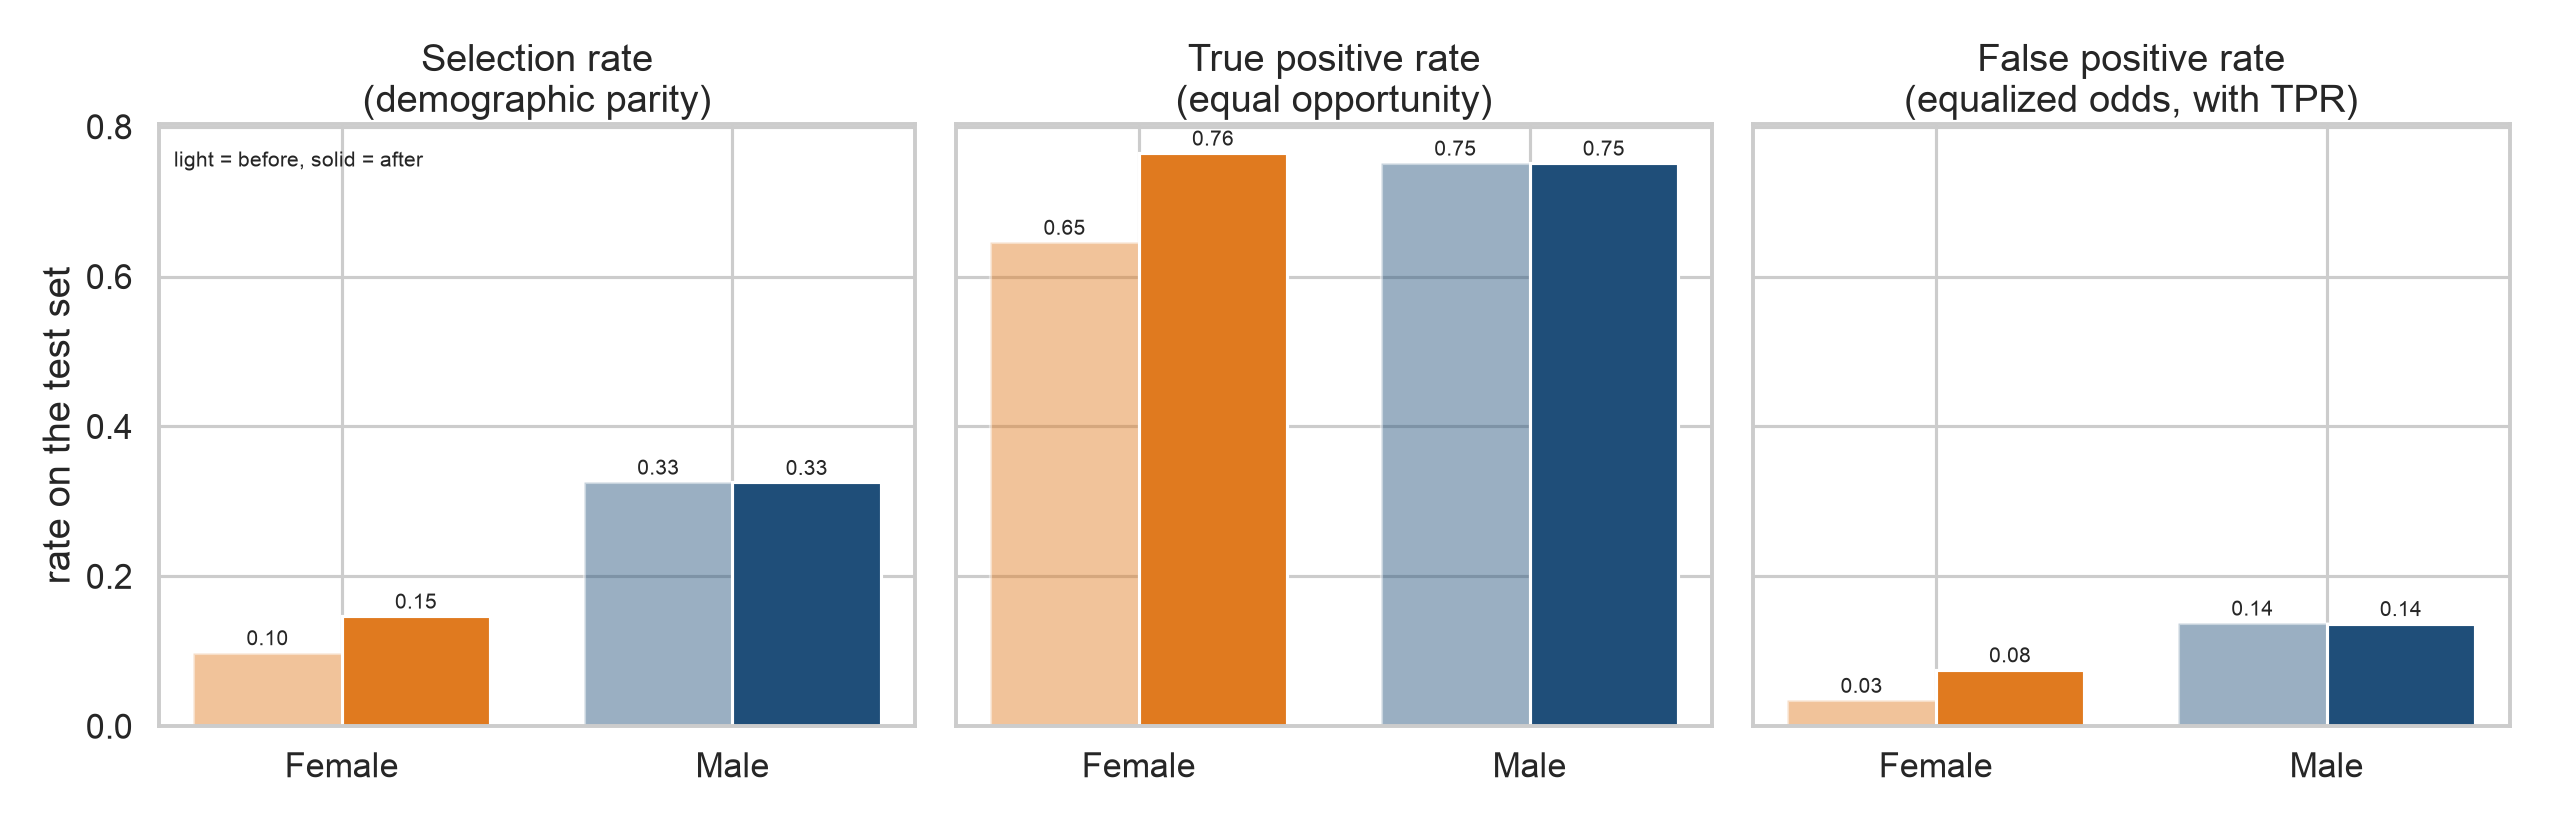
\includegraphics[width=0.92\linewidth]{fairness.png}
\caption{Rates by sex on the test set, before (light) and after (solid) mitigation.}\label{fig:fair}
\end{figure}

\paragraph{Reading.} Removing the attribute barely helps (EO gap 0.106 to 0.085): \code{relationship}
and \code{marital-status} are proxies, so the model reconstructs sex. Group thresholds reduce the
equal-opportunity gap from 0.106 to 0.013 in absolute value (the female TPR goes from 0.646 to 0.765,
slightly above the male 0.752), and the equalized-odds gap from 0.106 to 0.062. The cost is small:
$-0.007$ F1 and $-0.008$ accuracy; precision for women falls from 0.69 to 0.54, which is the price of
finding more of them. The demographic-parity gap remains large (0.178) because it reflects the base
rates, which no threshold should erase. Two limits: using a different threshold per sex is explicit
differential treatment, which is illegal in some uses (credit, hiring), so the endpoint serves
the single threshold by default and the group thresholds are documented as an option; and the
residual 0.013 shows that a threshold tuned on validation does not transfer perfectly.

\section{Serving, limits and conclusion}

\paragraph{Served endpoint.} \code{src/serve.py} exposes the final Pipeline with FastAPI:
\code{POST /predict} takes one raw record as JSON (validated by a Pydantic schema, missing values
allowed) and returns the probability, the decision and the threshold; \code{GET /health} returns the
model in use. The endpoint is covered by tests (valid request, rejected invalid request).

\paragraph{Limits.} The data is from 1994 and US-only: the 50K threshold, the labour market and the
gender gap have changed, so the model is a proof of concept and not a tool to use today. The model
relies heavily on capital gains and on marriage, a social proxy. The label is binary, so we cannot
tell 51K from 500K. Thresholds were chosen for F1, not for a real cost matrix.

\paragraph{Conclusion.} On a tabular, imbalanced problem, a disciplined pipeline matters more than
the choice of algorithm: going from logistic regression to tuned boosting buys 0.05 PR-AUC, while
a careless choice (default forest, class weights) costs as much in ranking or calibration. The final
model ranks well (PR-AUC 0.819, ROC-AUC 0.926), gives probabilities that can be trusted (ECE 0.007),
is explainable, and its main fairness gap can be closed for less than one point of F1.

\section*{Contribution statement}
\begin{table}[H]\centering\small
\begin{tabular}{lll}\toprule
Member & Technical requirements & Role\\\midrule
Amine Ennadzim & 1 EDA \& framing, 2 feature engineering, 5 Pipeline & data lead\\
Manuel Andrade & 3 class imbalance, 4 modelling progression & modelling lead\\
Gr\'egoire Mismaque & 6 Optuna tuning, 7 run log, 9 calibration & tuning and evaluation lead\\
Lucas Petrelluzzi & 8 explainability, 10 fairness audit, endpoint & responsible-AI lead, repository\\\bottomrule
\end{tabular}
\end{table}
\noindent Every member reviewed the whole report and can defend every part.

\appendix
\section{Run log}\label{app:runlog}
\begin{sloppypar}
The complete log is the supplementary file \code{runs/run\_log.csv} (110 lines, one per trial).
Columns: \code{run\_id}, \code{timestamp}, \code{model}, \code{trial}, \code{params} (JSON),
\code{cv\_pr\_auc\_mean}, \code{cv\_pr\_auc\_std}, \code{cv\_roc\_auc\_mean}, \code{cv\_brier\_mean},
\code{fit\_seconds}, \code{is\_best}, \code{artifact\_model}, \code{artifact\_plot}.
Every trial points to its own fitted pipeline
(\code{artifacts/models/trials/<model>\_trial<k>.joblib}, the configuration of the trial refitted
on the whole training set) and to the history plot of its study
(\code{reports/figures/optuna\_<model>.png}). The model of the best trial is copied to
\code{artifacts/models/<model>\_best.joblib}, the file evaluated in Section~\ref{sec:models}.
The 110 model files weigh several hundred megabytes, so they are not versioned:
\code{python main.py tune} regenerates them, with the same seed and the same results.
\end{sloppypar}

\begin{table}[H]\centering\footnotesize
\begin{tabular}{lrp{7.6cm}rrr}\toprule
Model & Trial & Parameters & CV PR-AUC & Std & CV Brier\\\midrule
logreg & 20* & $C=0.652$, L1 & 0.7839 & 0.0070 & 0.0986\\
logreg & 21 & $C=0.637$, L1 & 0.7839 & 0.0070 & 0.0986\\
logreg & 14 & $C=0.983$, L1 & 0.7839 & 0.0070 & 0.0986\\\midrule
random\_forest & 25* & 250 trees, depth 13, leaf 1, max\_features 0.43 & 0.8170 & 0.0050 & 0.0916\\
random\_forest & 26 & 250 trees, depth 12, leaf 1, max\_features 0.51 & 0.8165 & 0.0056 & 0.0916\\
random\_forest & 28 & 300 trees, depth 14, leaf 1, max\_features 0.36 & 0.8160 & 0.0045 & 0.0919\\\midrule
hist\_gb & 36* & lr 0.091, 450 iter, 14 leaves, leaf 78, L2 1.24, max\_features 0.60 & 0.8319 & 0.0058 & 0.0874\\
hist\_gb & 14 & lr 0.068, 500 iter, 11 leaves, leaf 70, L2 0.51, max\_features 0.52 & 0.8319 & 0.0055 & 0.0874\\
hist\_gb & 26 & lr 0.110, 550 iter, 17 leaves, leaf 70, L2 3.21, max\_features 0.68 & 0.8318 & 0.0058 & 0.0875\\\bottomrule
\end{tabular}
\caption{Three best trials per model (* = best trial of its study). Range over all
trials: logistic regression 0.718--0.784, random forest 0.794--0.817, gradient boosting 0.825--0.832.}
\end{table}

\begin{figure}[H]\centering
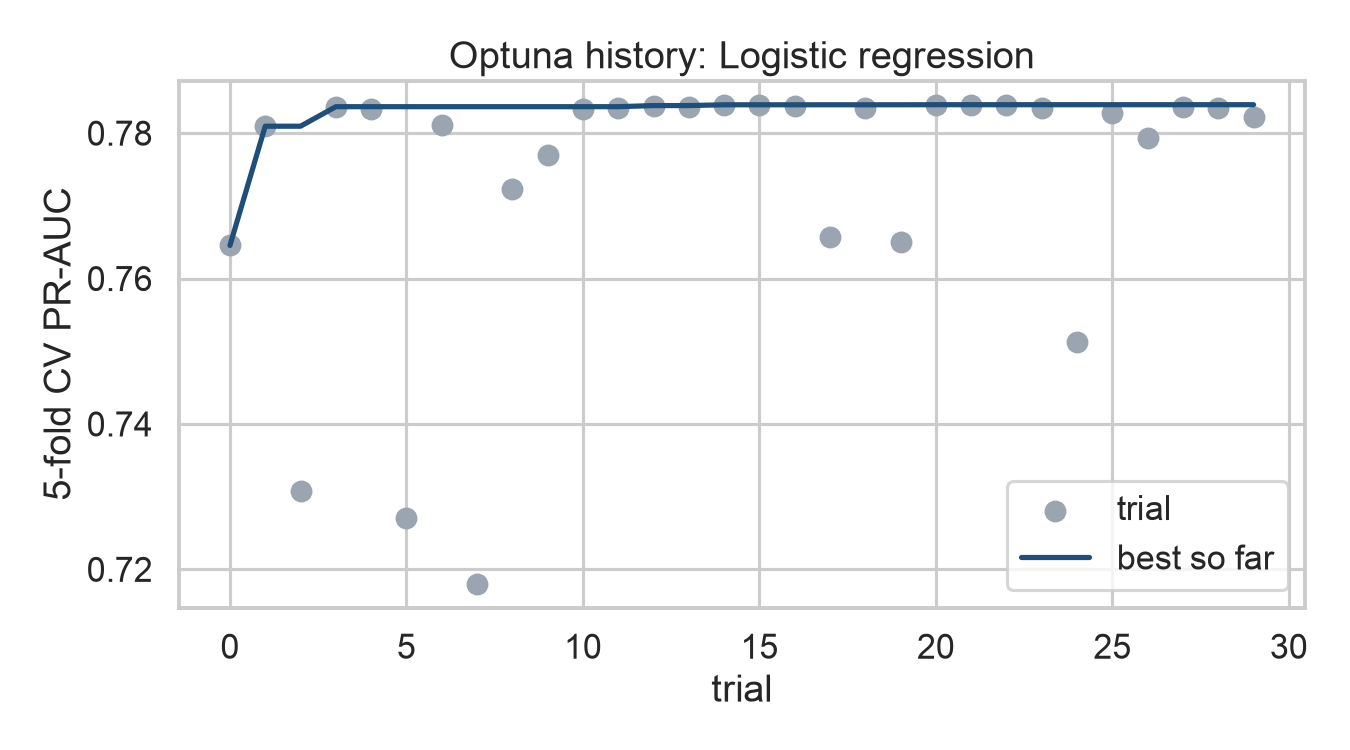
\includegraphics[width=0.32\linewidth]{optuna_logreg.png}\hfill
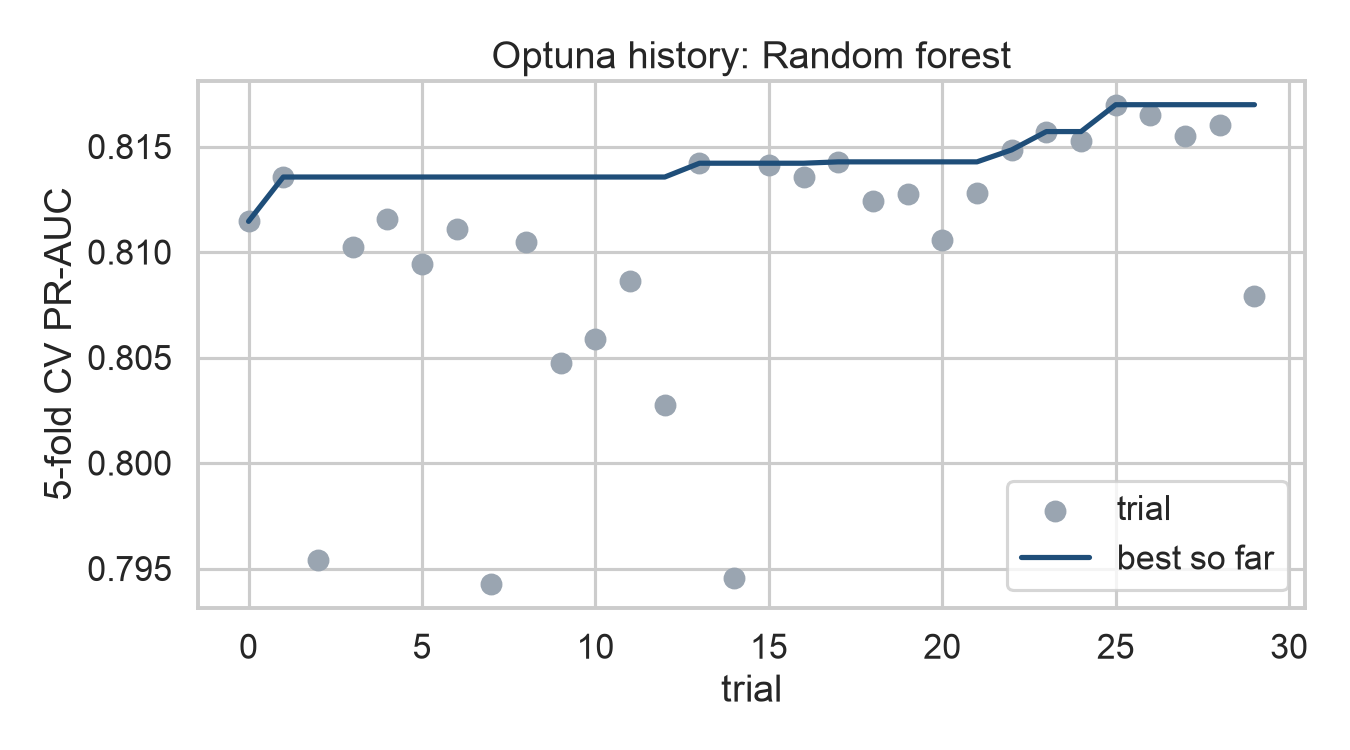
\includegraphics[width=0.32\linewidth]{optuna_random_forest.png}\hfill
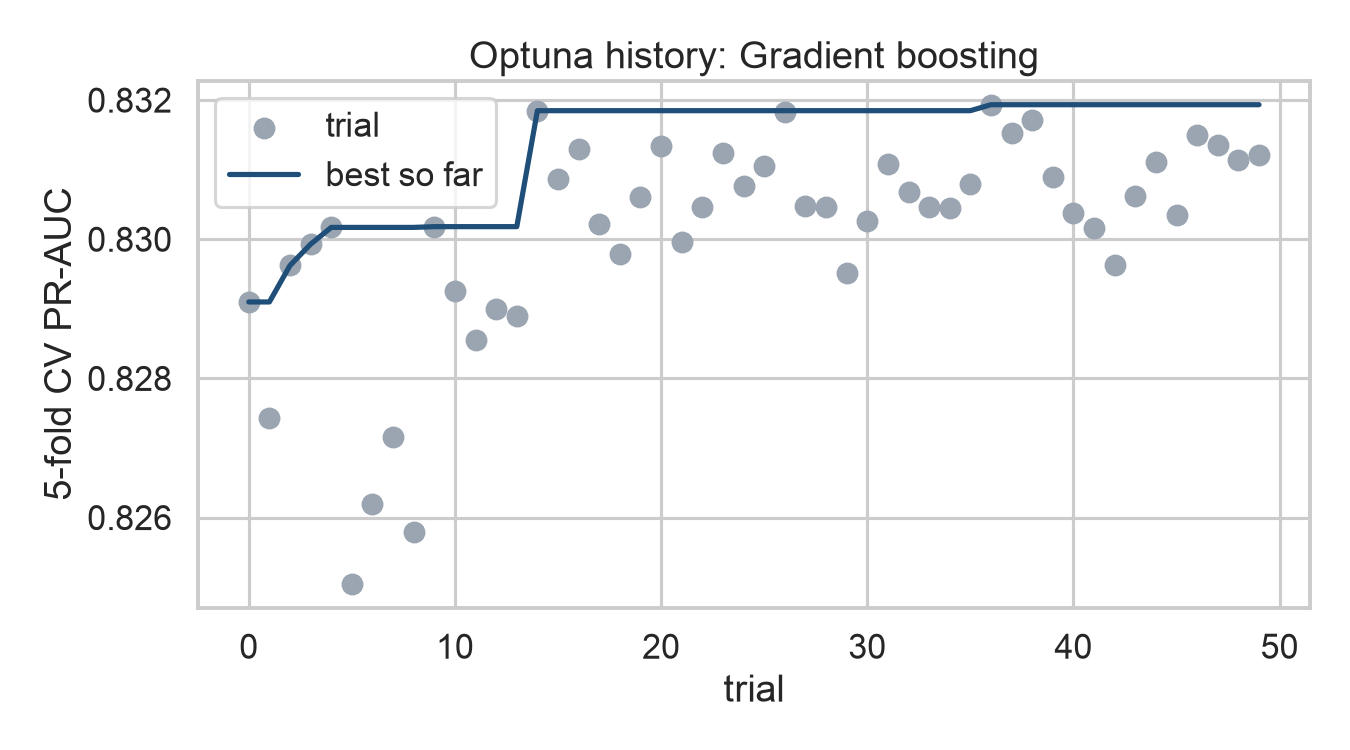
\includegraphics[width=0.32\linewidth]{optuna_hist_gb.png}
\caption{Optuna histories (5-fold CV PR-AUC per trial and best so far).}
\end{figure}

\section{Additional figures}
\begin{figure}[H]\centering
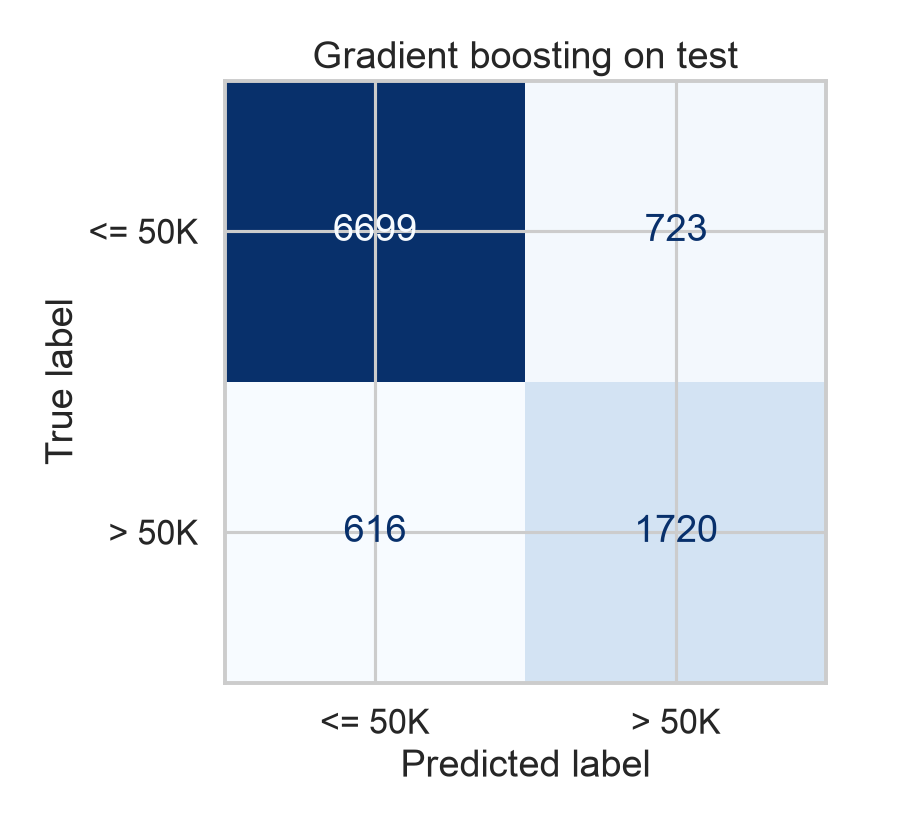
\includegraphics[width=0.36\linewidth]{confusion_matrix.png}\hfill
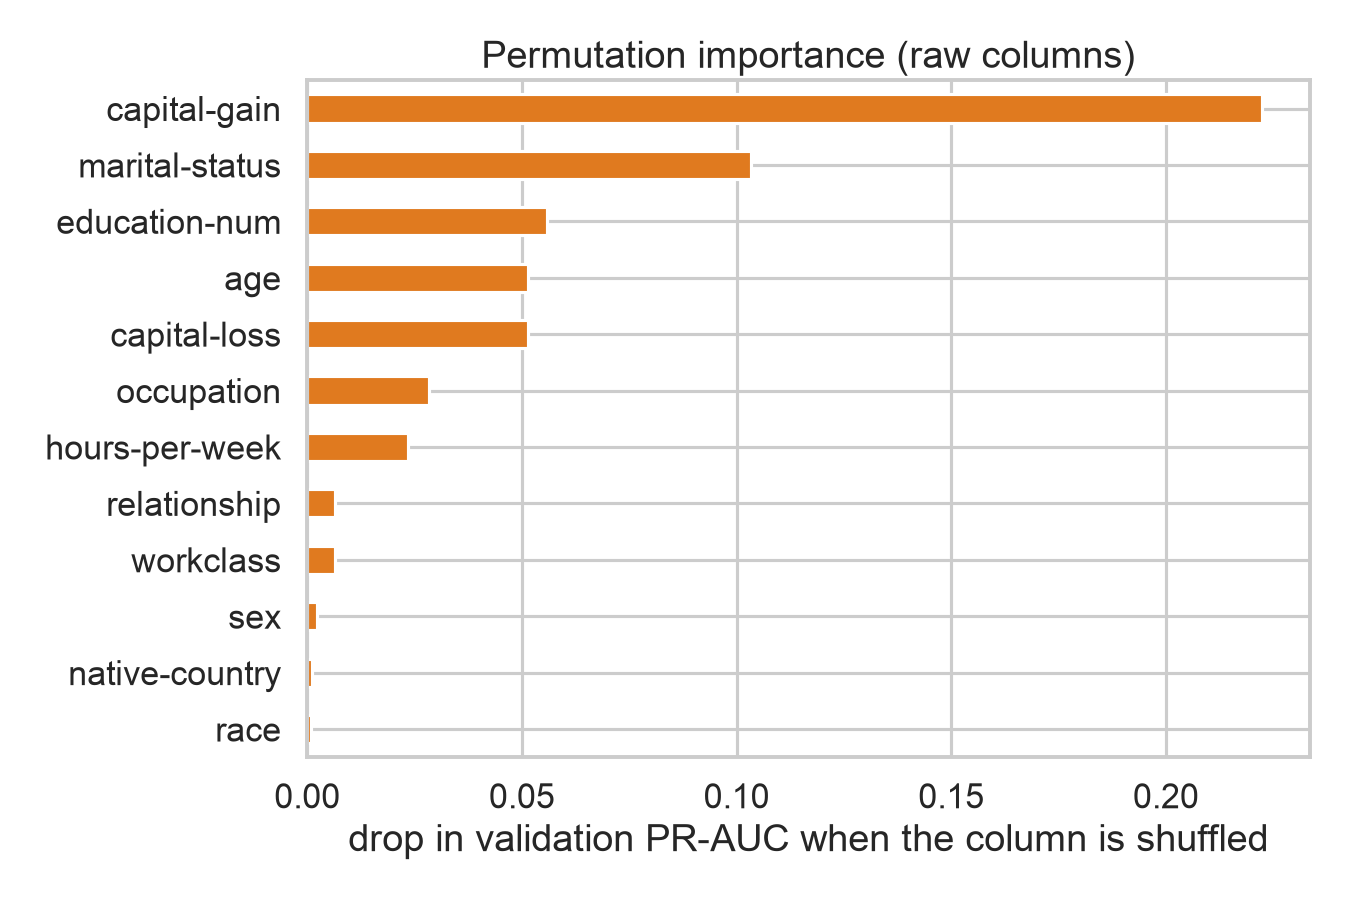
\includegraphics[width=0.56\linewidth]{permutation_importance.png}
\caption{Confusion matrix of the final model on the test set, and permutation importance.}
\end{figure}
\begin{figure}[H]\centering
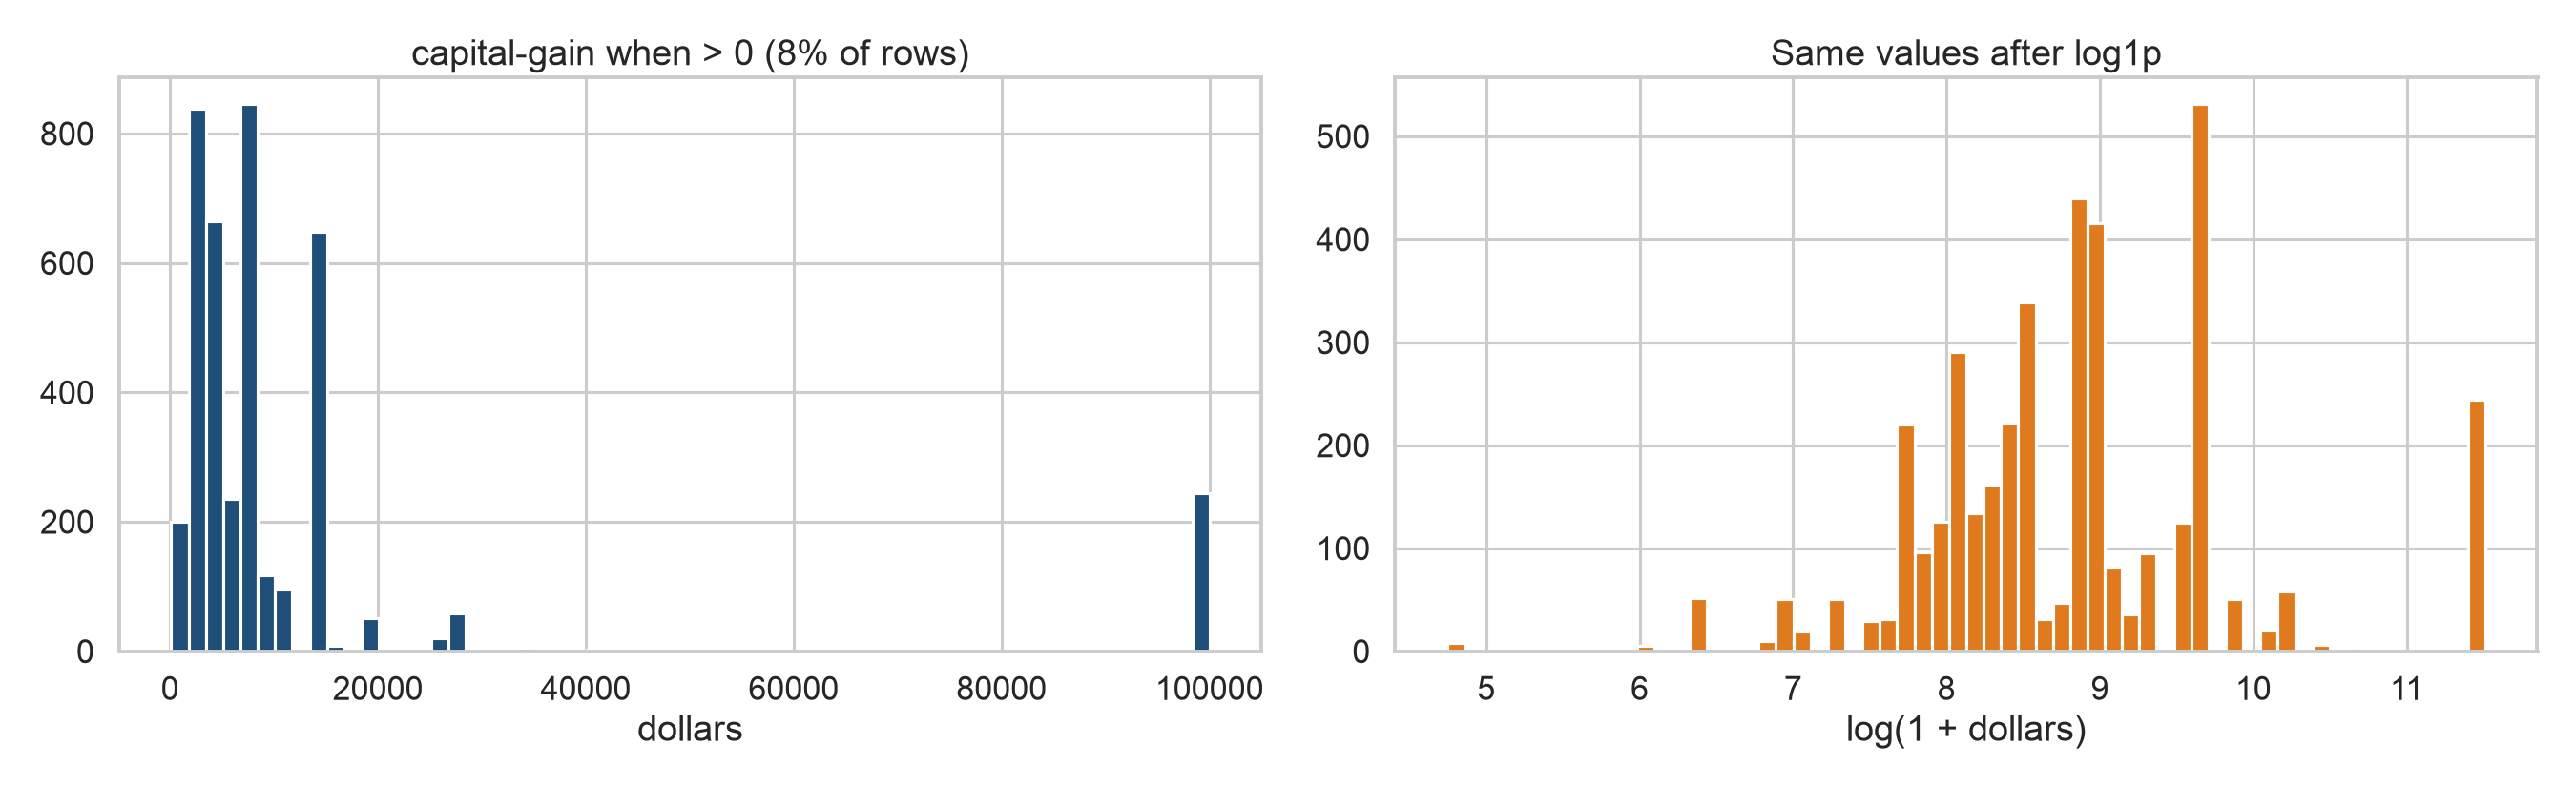
\includegraphics[width=0.8\linewidth]{eda_capital.png}
\caption{Capital gain before and after the log transformation.}
\end{figure}

\end{document}
